% Options for packages loaded elsewhere
% Options for packages loaded elsewhere
\PassOptionsToPackage{unicode}{hyperref}
\PassOptionsToPackage{hyphens}{url}
\PassOptionsToPackage{dvipsnames,svgnames,x11names}{xcolor}
%
\documentclass[
  11pt,
  letterpaper,
  DIV=11,
  numbers=noendperiod]{scrreprt}
\usepackage{xcolor}
\usepackage[margin=1in]{geometry}
\usepackage{amsmath,amssymb}
\setcounter{secnumdepth}{5}
\usepackage{iftex}
\ifPDFTeX
  \usepackage[T1]{fontenc}
  \usepackage[utf8]{inputenc}
  \usepackage{textcomp} % provide euro and other symbols
\else % if luatex or xetex
  \usepackage{unicode-math} % this also loads fontspec
  \defaultfontfeatures{Scale=MatchLowercase}
  \defaultfontfeatures[\rmfamily]{Ligatures=TeX,Scale=1}
\fi
\usepackage{lmodern}
\ifPDFTeX\else
  % xetex/luatex font selection
\fi
% Use upquote if available, for straight quotes in verbatim environments
\IfFileExists{upquote.sty}{\usepackage{upquote}}{}
\IfFileExists{microtype.sty}{% use microtype if available
  \usepackage[]{microtype}
  \UseMicrotypeSet[protrusion]{basicmath} % disable protrusion for tt fonts
}{}
\makeatletter
\@ifundefined{KOMAClassName}{% if non-KOMA class
  \IfFileExists{parskip.sty}{%
    \usepackage{parskip}
  }{% else
    \setlength{\parindent}{0pt}
    \setlength{\parskip}{6pt plus 2pt minus 1pt}}
}{% if KOMA class
  \KOMAoptions{parskip=half}}
\makeatother
% Make \paragraph and \subparagraph free-standing
\makeatletter
\ifx\paragraph\undefined\else
  \let\oldparagraph\paragraph
  \renewcommand{\paragraph}{
    \@ifstar
      \xxxParagraphStar
      \xxxParagraphNoStar
  }
  \newcommand{\xxxParagraphStar}[1]{\oldparagraph*{#1}\mbox{}}
  \newcommand{\xxxParagraphNoStar}[1]{\oldparagraph{#1}\mbox{}}
\fi
\ifx\subparagraph\undefined\else
  \let\oldsubparagraph\subparagraph
  \renewcommand{\subparagraph}{
    \@ifstar
      \xxxSubParagraphStar
      \xxxSubParagraphNoStar
  }
  \newcommand{\xxxSubParagraphStar}[1]{\oldsubparagraph*{#1}\mbox{}}
  \newcommand{\xxxSubParagraphNoStar}[1]{\oldsubparagraph{#1}\mbox{}}
\fi
\makeatother

\usepackage{color}
\usepackage{fancyvrb}
\newcommand{\VerbBar}{|}
\newcommand{\VERB}{\Verb[commandchars=\\\{\}]}
\DefineVerbatimEnvironment{Highlighting}{Verbatim}{commandchars=\\\{\}}
% Add ',fontsize=\small' for more characters per line
\usepackage{framed}
\definecolor{shadecolor}{RGB}{241,243,245}
\newenvironment{Shaded}{\begin{snugshade}}{\end{snugshade}}
\newcommand{\AlertTok}[1]{\textcolor[rgb]{0.68,0.00,0.00}{#1}}
\newcommand{\AnnotationTok}[1]{\textcolor[rgb]{0.37,0.37,0.37}{#1}}
\newcommand{\AttributeTok}[1]{\textcolor[rgb]{0.40,0.45,0.13}{#1}}
\newcommand{\BaseNTok}[1]{\textcolor[rgb]{0.68,0.00,0.00}{#1}}
\newcommand{\BuiltInTok}[1]{\textcolor[rgb]{0.00,0.23,0.31}{#1}}
\newcommand{\CharTok}[1]{\textcolor[rgb]{0.13,0.47,0.30}{#1}}
\newcommand{\CommentTok}[1]{\textcolor[rgb]{0.37,0.37,0.37}{#1}}
\newcommand{\CommentVarTok}[1]{\textcolor[rgb]{0.37,0.37,0.37}{\textit{#1}}}
\newcommand{\ConstantTok}[1]{\textcolor[rgb]{0.56,0.35,0.01}{#1}}
\newcommand{\ControlFlowTok}[1]{\textcolor[rgb]{0.00,0.23,0.31}{\textbf{#1}}}
\newcommand{\DataTypeTok}[1]{\textcolor[rgb]{0.68,0.00,0.00}{#1}}
\newcommand{\DecValTok}[1]{\textcolor[rgb]{0.68,0.00,0.00}{#1}}
\newcommand{\DocumentationTok}[1]{\textcolor[rgb]{0.37,0.37,0.37}{\textit{#1}}}
\newcommand{\ErrorTok}[1]{\textcolor[rgb]{0.68,0.00,0.00}{#1}}
\newcommand{\ExtensionTok}[1]{\textcolor[rgb]{0.00,0.23,0.31}{#1}}
\newcommand{\FloatTok}[1]{\textcolor[rgb]{0.68,0.00,0.00}{#1}}
\newcommand{\FunctionTok}[1]{\textcolor[rgb]{0.28,0.35,0.67}{#1}}
\newcommand{\ImportTok}[1]{\textcolor[rgb]{0.00,0.46,0.62}{#1}}
\newcommand{\InformationTok}[1]{\textcolor[rgb]{0.37,0.37,0.37}{#1}}
\newcommand{\KeywordTok}[1]{\textcolor[rgb]{0.00,0.23,0.31}{\textbf{#1}}}
\newcommand{\NormalTok}[1]{\textcolor[rgb]{0.00,0.23,0.31}{#1}}
\newcommand{\OperatorTok}[1]{\textcolor[rgb]{0.37,0.37,0.37}{#1}}
\newcommand{\OtherTok}[1]{\textcolor[rgb]{0.00,0.23,0.31}{#1}}
\newcommand{\PreprocessorTok}[1]{\textcolor[rgb]{0.68,0.00,0.00}{#1}}
\newcommand{\RegionMarkerTok}[1]{\textcolor[rgb]{0.00,0.23,0.31}{#1}}
\newcommand{\SpecialCharTok}[1]{\textcolor[rgb]{0.37,0.37,0.37}{#1}}
\newcommand{\SpecialStringTok}[1]{\textcolor[rgb]{0.13,0.47,0.30}{#1}}
\newcommand{\StringTok}[1]{\textcolor[rgb]{0.13,0.47,0.30}{#1}}
\newcommand{\VariableTok}[1]{\textcolor[rgb]{0.07,0.07,0.07}{#1}}
\newcommand{\VerbatimStringTok}[1]{\textcolor[rgb]{0.13,0.47,0.30}{#1}}
\newcommand{\WarningTok}[1]{\textcolor[rgb]{0.37,0.37,0.37}{\textit{#1}}}

\usepackage{longtable,booktabs,array}
\usepackage{calc} % for calculating minipage widths
% Correct order of tables after \paragraph or \subparagraph
\usepackage{etoolbox}
\makeatletter
\patchcmd\longtable{\par}{\if@noskipsec\mbox{}\fi\par}{}{}
\makeatother
% Allow footnotes in longtable head/foot
\IfFileExists{footnotehyper.sty}{\usepackage{footnotehyper}}{\usepackage{footnote}}
\makesavenoteenv{longtable}
\usepackage{graphicx}
\makeatletter
\newsavebox\pandoc@box
\newcommand*\pandocbounded[1]{% scales image to fit in text height/width
  \sbox\pandoc@box{#1}%
  \Gscale@div\@tempa{\textheight}{\dimexpr\ht\pandoc@box+\dp\pandoc@box\relax}%
  \Gscale@div\@tempb{\linewidth}{\wd\pandoc@box}%
  \ifdim\@tempb\p@<\@tempa\p@\let\@tempa\@tempb\fi% select the smaller of both
  \ifdim\@tempa\p@<\p@\scalebox{\@tempa}{\usebox\pandoc@box}%
  \else\usebox{\pandoc@box}%
  \fi%
}
% Set default figure placement to htbp
\def\fps@figure{htbp}
\makeatother


% definitions for citeproc citations
\NewDocumentCommand\citeproctext{}{}
\NewDocumentCommand\citeproc{mm}{%
  \begingroup\def\citeproctext{#2}\cite{#1}\endgroup}
\makeatletter
 % allow citations to break across lines
 \let\@cite@ofmt\@firstofone
 % avoid brackets around text for \cite:
 \def\@biblabel#1{}
 \def\@cite#1#2{{#1\if@tempswa , #2\fi}}
\makeatother
\newlength{\cslhangindent}
\setlength{\cslhangindent}{1.5em}
\newlength{\csllabelwidth}
\setlength{\csllabelwidth}{3em}
\newenvironment{CSLReferences}[2] % #1 hanging-indent, #2 entry-spacing
 {\begin{list}{}{%
  \setlength{\itemindent}{0pt}
  \setlength{\leftmargin}{0pt}
  \setlength{\parsep}{0pt}
  % turn on hanging indent if param 1 is 1
  \ifodd #1
   \setlength{\leftmargin}{\cslhangindent}
   \setlength{\itemindent}{-1\cslhangindent}
  \fi
  % set entry spacing
  \setlength{\itemsep}{#2\baselineskip}}}
 {\end{list}}
\usepackage{calc}
\newcommand{\CSLBlock}[1]{\hfill\break\parbox[t]{\linewidth}{\strut\ignorespaces#1\strut}}
\newcommand{\CSLLeftMargin}[1]{\parbox[t]{\csllabelwidth}{\strut#1\strut}}
\newcommand{\CSLRightInline}[1]{\parbox[t]{\linewidth - \csllabelwidth}{\strut#1\strut}}
\newcommand{\CSLIndent}[1]{\hspace{\cslhangindent}#1}



\setlength{\emergencystretch}{3em} % prevent overfull lines

\providecommand{\tightlist}{%
  \setlength{\itemsep}{0pt}\setlength{\parskip}{0pt}}



 


\usepackage{booktabs}
\usepackage{longtable}
\usepackage{array}
\usepackage{multirow}
\usepackage{wrapfig}
\usepackage{float}
\usepackage{colortbl}
\usepackage{pdflscape}
\usepackage{tabu}
\usepackage{threeparttable}
\usepackage{threeparttablex}
\usepackage[normalem]{ulem}
\usepackage{makecell}
\usepackage{xcolor}
\KOMAoption{captions}{tableheading,figureheading}
\makeatletter
\@ifpackageloaded{tcolorbox}{}{\usepackage[skins,breakable]{tcolorbox}}
\@ifpackageloaded{fontawesome5}{}{\usepackage{fontawesome5}}
\definecolor{quarto-callout-color}{HTML}{909090}
\definecolor{quarto-callout-note-color}{HTML}{0758E5}
\definecolor{quarto-callout-important-color}{HTML}{CC1914}
\definecolor{quarto-callout-warning-color}{HTML}{EB9113}
\definecolor{quarto-callout-tip-color}{HTML}{00A047}
\definecolor{quarto-callout-caution-color}{HTML}{FC5300}
\definecolor{quarto-callout-color-frame}{HTML}{acacac}
\definecolor{quarto-callout-note-color-frame}{HTML}{4582ec}
\definecolor{quarto-callout-important-color-frame}{HTML}{d9534f}
\definecolor{quarto-callout-warning-color-frame}{HTML}{f0ad4e}
\definecolor{quarto-callout-tip-color-frame}{HTML}{02b875}
\definecolor{quarto-callout-caution-color-frame}{HTML}{fd7e14}
\makeatother
\makeatletter
\@ifpackageloaded{bookmark}{}{\usepackage{bookmark}}
\makeatother
\makeatletter
\@ifpackageloaded{caption}{}{\usepackage{caption}}
\AtBeginDocument{%
\ifdefined\contentsname
  \renewcommand*\contentsname{Table of contents}
\else
  \newcommand\contentsname{Table of contents}
\fi
\ifdefined\listfigurename
  \renewcommand*\listfigurename{List of Figures}
\else
  \newcommand\listfigurename{List of Figures}
\fi
\ifdefined\listtablename
  \renewcommand*\listtablename{List of Tables}
\else
  \newcommand\listtablename{List of Tables}
\fi
\ifdefined\figurename
  \renewcommand*\figurename{Figure}
\else
  \newcommand\figurename{Figure}
\fi
\ifdefined\tablename
  \renewcommand*\tablename{Table}
\else
  \newcommand\tablename{Table}
\fi
}
\@ifpackageloaded{float}{}{\usepackage{float}}
\floatstyle{ruled}
\@ifundefined{c@chapter}{\newfloat{codelisting}{h}{lop}}{\newfloat{codelisting}{h}{lop}[chapter]}
\floatname{codelisting}{Listing}
\newcommand*\listoflistings{\listof{codelisting}{List of Listings}}
\makeatother
\makeatletter
\makeatother
\makeatletter
\@ifpackageloaded{caption}{}{\usepackage{caption}}
\@ifpackageloaded{subcaption}{}{\usepackage{subcaption}}
\makeatother
\usepackage{bookmark}
\IfFileExists{xurl.sty}{\usepackage{xurl}}{} % add URL line breaks if available
\urlstyle{same}
\hypersetup{
  pdftitle={Comparing LLM and human reviews of social science research using data from Unjournal.org},
  pdfauthor={Valentin Klotzbücher; David Reinstein; Lorenzo Pacchiardi; Tianmai Michael Zhang},
  colorlinks=true,
  linkcolor={blue},
  filecolor={Maroon},
  citecolor={Blue},
  urlcolor={Blue},
  pdfcreator={LaTeX via pandoc}}


\title{Comparing LLM and human reviews of social science research using
data from Unjournal.org}
\author{Valentin Klotzbücher \and David Reinstein \and Lorenzo
Pacchiardi \and Tianmai Michael Zhang}
\date{2026-02-15}
\begin{document}
\maketitle
\begin{abstract}
We benchmark how frontier LLMs critique, rate, and prioritize research,
comparing AI-generated evaluations to human expert assessments from The
Unjournal. Human ratings serve as a reference signal---the core goal is
measuring and diagnosing AI reasoning quality: understanding
calibration, failure modes, and systematic ``taste'' differences between
AI and human evaluators.
\end{abstract}

\renewcommand*\contentsname{Table of contents}
{
\hypersetup{linkcolor=}
\setcounter{tocdepth}{2}
\tableofcontents
}

\bookmarksetup{startatroot}

\chapter{Introduction}\label{introduction}

\begin{tcolorbox}[enhanced jigsaw, colback=white, title=\textcolor{quarto-callout-note-color}{\faInfo}\hspace{0.5em}{Working paper}, bottomrule=.15mm, coltitle=black, left=2mm, colframe=quarto-callout-note-color-frame, toptitle=1mm, toprule=.15mm, titlerule=0mm, breakable, leftrule=.75mm, colbacktitle=quarto-callout-note-color!10!white, bottomtitle=1mm, arc=.35mm, rightrule=.15mm, opacityback=0, opacitybacktitle=0.6]

This is an evolving working paper. Analysis, metrics, and comparisons
are under active development.

\end{tcolorbox}

Is AI good at peer-reviewing? Does it offer useful and valid feedback?
Can it predict how human experts will rate research across a range of
categories? How can it help academics do this ``thankless'' task better?
Is it particularly good at spotting errors? Are there specific
categories, e.g.~spotting math errors or judging real-world relevance,
where it does surprisingly well or poorly? How does its ``research
taste'' compare to humans?

If AI research-evaluation works it could free up a lot of scientific
resources -- perhaps \$1.5 billion/year in the US alone
(\citeproc{ref-aczel2021billion}{Aczel, Szaszi, and Holcombe 2021}) --
and offer more continual and detailed review, helping improve research
and address the
``\href{https://www.nature.com/articles/d41586-025-02457-2}{peer-review
crisis}''. Numerous accounts report a system under strain, with
widespread difficulty finding human peer reviewers with appropriate
expertise willing to put in careful effort. An influx of AI-generated or
AI-human hybrid research seems likely to exacerbate this
problem.\footnote{E.g., see
  \href{https://www.linkedin.com/feed/update/urn:li:activity:7411759911480524800/}{anectodal
  reports}. Proposed solutions include a credit or payment-based model.
  (Further references to be added.).} AI research evaluation could also
help characterize methodological strengths and weaknesses across papers,
aiding research training and research direction-setting.

Furthermore,
``\href{https://www.nytimes.com/2025/12/26/podcasts/hardfork-ai-science.html}{the
leaders of the biggest A.I. labs} argue that artificial intelligence
will usher in a new era of scientific discovery, which will help us cure
diseases and accelerate our ability to address the climate crisis'' --
e.g., Sam Altman on
\href{https://blog.samaltman.com/abundant-intelligence}{cures for
cancer}, etc. Understanding how AI engages with research evaluations may
provide a window into its values, abilities, and limitations.\footnote{Eger
  et al. (\citeproc{ref-eger2025}{2025}): ``When it comes to using AI
  tools for science, ethics is of overarching importance. This is
  because the AI tools exhibit various limitations, e.g., they (i) may
  hallucinate and fabricate content, (ii) exhibit bias, (iii) may have
  limited reasoning abilities and (iv) sometimes lack suitable
  evaluation, \ldots{} among many other concerns such as risks of fake
  science, plagiarism, and lack of human authority. Indeed, the European
  Union has recently released guidelines on the responsible use of AI
  for science. In it, it points out that, while''{[}r{]}esearch is one
  of the sectors that could be most significantly disrupted by
  generative AI'' where ``AI has great potential for accelerating
  scientific discovery and improving the effectiveness and pace of
  research and verification processes''}

In this project, we pilot the use of The Unjournal's evaluations as a
benchmark to test the capabilities of current large language models
(LLMs) and bespoke agent-based tools, considering how the research
evaluations these generate compare to expert human reviews. The
Unjournal systematically prioritizes `impactful' research and pays for
high-quality human evaluations, structured quantified ratings, claim
identification and assessment, and predictions. They further labeled and
classified ``major consensus critiques'' from a subset of these
evaluations.\footnote{An individual rater (David Reinstein, Co-director
  of The Unjournal) curated a pilot version of this
  \href{https://coda.io/d/Unjournal-Public-Pages_ddIEzDONWdb/Piloting-a-benchmark-rubric-for-LLM-tools-Public_su7jCZTB\#_luqSuSgh}{here},
  focusing on critiques identified by multiple evaluators and/or
  confirmed by the author or evaluation manager. We are currently (Jan
  5, 2026) comparing this enumeration to the issues identified by LLM's
  (see ``Results: Critiques'' chapter). Future work will systematically
  employ multiple enumerators with a pre-defined rubric.}

We next prompt several LLMs and agent-based tools\footnote{Dec 2025
  focus: OpenAI's GPT-5.2 Pro model} to review the same set of
quantitative social science research evaluated by The Unjournal's human
evaluators, with the same set of criteria and guidelines. Each paper is
assessed on specific dimensions -- for example, the strength of its
evidence, rigor of methods, clarity of communication,
openness/reproducibility, relevance to global priorities, and overall
quality. The LLM will provide quantitative scores (with uncertainty
intervals) on these criteria and produce a written evaluation.

Our initial dataset will include the 60 research papers that have
existing Unjournal human evaluations.\footnote{This is slightly off as
  of January 2026. We only have 56 papers with official Unjournal
  evaluations. I suspect this data includes some papers that are either
  duplicated or in our pipeline for given an independent non-official
  evaluation} For each paper, the AI will generate: (1) numeric ratings
on the defined criteria, (2) identification of the paper's key claims,
and (3) a detailed review enumerating and discussing the paper's
contributions and weaknesses. We then compare the AI-generated
evaluations to the published human evaluations, considering both
quantitative metrics (e.g., inter-rater reliability), identification of
consensus critiques, and qualitative comparison. The next phase will
train and tune models, and measure their performance on research
currently in The Unjournal's pipeline, i.e., where no human evaluation
has yet been made public, to enable out-of-time validation, confirmatory
hypothesis tests, and less risk of model contamination.

This complements other recent work on AI-evaluation approaches and
benchmarks, outlined below. Our work offers in-depth comparisons and
oversight in a high-nuance and high-value context:
global-priorities-relevant economics and social-science research, and
leverages The Unjournal's ongoing pipeline as a continual experimental
and feedback environment.

\section{Research Goals and Questions
(overview)}\label{research-goals-and-questions-overview}

\begin{enumerate}
\def\labelenumi{\arabic{enumi}.}
\tightlist
\item
  \textbf{Measure the value of frontier AI research evaluation vs.~human
  peer review}

  \begin{itemize}
  \tightlist
  \item
    Is state-of-the-art AI research evaluation reliable and useful
    enough to replace human peer review in these contexts?
  \item
    Reverse question: The Unjournal was asked -- ``Are \emph{human}
    evaluations worth it''?
  \item
    How well can AI predict what humans will report?
  \item
    What are AI's strengths \& weaknesses relative to humans, e.g., in
    terms of: (1) Predicting journal outcomes, citations, etc. (2)
    Generating feedback deemed most useful by humans (3) Spotting
    research errors (4) Diagnosing different types of strengths and
    limitations (e.g., reasoning transparency, justification of methods
    and assumptions, communication) (5) Judging content without
    biases/statistical discrimination based on prestige labels, etc.
  \end{itemize}
\item
  \textbf{Compare methods for AI research-evaluation, find the best
  approaches}

  \begin{itemize}
  \tightlist
  \item
    Which approaches come closest to (the desirable features of) human
    evaluations and in which ways?
  \item
    What gets closest to the `frontier', doing better in terms of
    outcomes like those mentioned above?
  \end{itemize}
\item
  \textbf{The nature of frontier AI `preferences \& tastes' over
  research}

  \begin{itemize}
  \tightlist
  \item
    Which types of papers and approaches do default models tend to
    `like' more/less relative to humans when given the same guidelines?
  \item
    Do we see signs of characteristic preferences that help us
    understand how AIs are likely to prioritize, conduct, and evaluate
    research?
  \end{itemize}
\item
  \textbf{Hybrid human-AI performance} (future trials)
\end{enumerate}

\section{Our work in context}\label{sec-our-work-in-context}

\subsection[AI practical research applications]{\texorpdfstring{AI
practical research
applications\footnote{We maintain a NotebookLM of the most relevant and
  related research
  \href{https://notebooklm.google.com/notebook/f4dde07a-a1bc-470d-93b2-052a3c795933}{here}.}}{AI practical research applications}}\label{ai-practical-research-applicationsindex-6}

Luo et al. (\citeproc{ref-Luo2025}{2025}) survey LLM roles from idea
generation to peer review, including experiment planning and automated
scientific writing. They highlight opportunities (productivity, coverage
of long documents) alongside governance needs (provenance, detection of
LLM-generated content, standardizing tooling) and call for reliable
evaluation frameworks.

Korinek (\citeproc{ref-korinek2025ai}{2025}) considers the specific
potential for using AI in economic research, offering ``working examples
and step-by-step code'' to help economists use agents for literature
reviews, econometric code, fetching and analyzing economic data, and
coordinate complex research workflows. He advocates economists using AI
tools to boost productivity and ``to understand {[}these tools'{]}
capabilities and limitations.'' He calls for human researcher oversight
``to ensure {[}these tools{]} pursue the right objectives and maintain
research integrity''. He outlines a range of current limitations and
open questions (outlined
\href{https://docs.google.com/document/d/1CVNnG6Jw3gr1sbI9Z_vIIJ1BI9O-8-Eev6D2j22vaeg/edit?tab=t.0\#heading=h.9pcc2azfjlro}{here}),
including hallucinations, mistakes compounding through multi-agent
workflows and ``brittleness to small variations in prompts''. At the
higher level, he argues ``the questions that will matter most---what
problems deserve investigation, how should we evaluate trade-offs, what
constitutes progress---will remain irreducibly human.''

Mitchener, Yiu, et al. (\citeproc{ref-mitchener2025kosmos}{2025})
present Kosmos, ``an AI scientist for autonomous discovery''. However,
evaluations reveal important limitations:

\begin{itemize}
\item
  ``Kosmos was found to be only 57\% accurate in statements that
  required interpretation of results, likely due to its propensity to
  conflate statistically significant results with scientifically
  valuable ones''
\item
  ``although 85\% of statements derived from data analyses were
  accurate, our evaluations do not capture if the analyses Kosmos chose
  to execute were the ones most likely to yield novel or interesting
  scientific insights.''\ldots{} ``identifying valuable discoveries
  Kosmos made is a time-intensive process that relies on human
  scientists with significant domain expertise''
\end{itemize}

\subsection{AI peer review, error detection, and research
evaluation}\label{ai-peer-review-error-detection-and-research-evaluation}

Son et al. (\citeproc{ref-son2025flaws}{2025}) evaluates LLMs on 83
papers paired with 91 confirmed significant scientific errors. This
resembles our own approach, although they focus on
erratta/retraction-worthy errors, while we consider more nuanced
methodological limitations. Their strongest (OpenAI o3) model identified
only 21.1\% of these errors, with only 6.1\% precision.\footnote{They
  asked domain experts to do qualitative analysis, which found most
  false positives were hallucinations or student-level misconceptions}

Eger et al. (\citeproc{ref-eger2025}{2025}) provide a broad review of
LLMs in science and a focused discussion of AI‑assisted peer review.
They argue: (i) peer‑review data is scarce and concentrated in
CS/OpenReview venues; (ii) targeted assistance that preserves human
autonomy is preferable to end‑to‑end reviewing; and (iii) ethics and
governance (bias, provenance, detection of AI‑generated text) are
first‑class constraints.

Dycke, Kuznetsov, and Gurevych (\citeproc{ref-dycke2023}{2023}) present
NLPEER, a ``multidomain corpus'' of more than 5000 papers and 11k review
reports from 2012 to 2022 from five different venues''.

Zhang and Abernethy (\citeproc{ref-Zhang2025}{2025}) propose deploying
LLMs as quality checkers to surface critical problems instead of
generating full narrative reviews. Using papers from WITHDRARXIV and an
automatic evaluation framework that leverages ``LLM-as-judge,'' they
find the best performance from top reasoning models but still recommend
human oversight.

Pataranutaporn et al. (\citeproc{ref-Pataranutaporn2025}{2025}) asked
four nearly state-of-the-art LLM models (GPT-4o mini, Claude 3.5 Haiku,
Gemma 3 27B, and LLaMA 3.3 70B) to consider 1220 unique papers ``drawn
from 110 economics journals excluded from the training data of current
LLMs''. They prompted the models to act ``in your capacity as a reviewer
for {[}a top-5 economics journal{]}'' and make a publication
recommendation using a 6-point scale ranging from ``1 = Definite
Reject\ldots{}'' to ``6. Accept As Is\ldots{}''. They asked it to
evaluate each paper on a 10-point scale for originality, rigor, scope,
impact, and whether it was `written by AI'. They also (separately) had
LLMs rate 330 papers with the authors' identities removed, or replacing
the names with fake male/female names and real elite or non-elite
institutions or with prominent male or female economists attached.

They compare the LLMs' ratings with the RePEC rankings for the journals
the papers were published in, finding general alignment. They find mixed
results on detecting AI-generated papers. In the names/institutions
comparisons, they also find the LLMs show biases towards named
high-prestige male authors relative to high-prestige female authors, as
well as biases towards elite institutions and US/UK universities.

There have been several other empirical benchmarking projects, including
work covered in LLM4SR: A Survey on Large Language Models for Scientific
Research and \href{https://arxiv.org/abs/2502.05151}{Transforming
Science with Large Language Models: A Survey on AI-assisted Scientific
Discovery, Experimentation, Content Generation, and Evaluation}. (See
cited surveys for additional benchmarks.)

Zhang et al. (\citeproc{ref-Zhang2025Replication}{2025}) use AI
conference paper data and LLM agents for pairwise manuscript
comparisons, finding this approach outperforms traditional rating-based
methods for identifying high-impact papers by citation metrics, though
with some evidence of biases favoring established research
institutions.\footnote{Key findings from Zhang et al.
  (\citeproc{ref-Zhang2025Replication}{2025}): (1) Uses AI conference
  paper data; (2) Employs LLM agents for pairwise manuscript
  comparisons; (3) Significantly outperforms traditional rating-based
  methods in identifying high-impact papers by citation metrics; (4)
  Shows some evidence of biases/statistical discrimination based on
  characteristics like `papers from established research institutions'.}

We discuss how our approach differs from prior work
\hyperref[sec-our-present-focus-the-unjournal-opportunity]{below}.\footnote{See
  below. Claude's brief summary ``Our approach differs from prior work
  by (i) focusing on structured, percentile-based quantitative ratings
  with credible intervals that map to decision-relevant dimensions used
  by The Unjournal; (ii) comparing those ratings to published human
  evaluations rather than using LLM-as-judge; and (iii) curating
  contamination-aware inputs (paper text extraction with
  reference-section removal and token caps), with a roadmap to add
  multi-modal checks when we score figure- or table-dependent
  criteria''.}

\subsection{AI research taste and potential to guide
research}\label{sec-ai-research-taste-and-potential-to-guide-research}

A key motivation for this work stems from broader claims about AI's
potential to accelerate scientific discovery and ``revolutionize
science.'' If AI systems are to contribute meaningfully to
research---not just as tools but as evaluators and potential
collaborators---we need to understand their ``taste'': what they value,
what they miss, and whether their priorities align with human expert
judgment and real-world research impact.

Understanding LLM preferences and blind spots when evaluating research
provides a window into:

\begin{itemize}
\tightlist
\item
  Whether AI can identify truly impactful research vs.~stylistic or
  superficial features
\item
  Potential systematic biases in how AI might direct future research
  priorities
\item
  The risks and opportunities of AI-assisted or AI-directed research
  agendas
\end{itemize}

This connects to broader debates about the returns to science in the
presence of technological risk (\citeproc{ref-clancy2023returns}{Clancy
2023}), where optimistic forecasts of AI-accelerated science must be
weighed against potential downsides and the question of whether AI
judgments align with what actually advances knowledge and improves
outcomes.

\subsection{Our present focus, The Unjournal
opportunity}\label{sec-our-present-focus-the-unjournal-opportunity}

Our project distinguishes itself through several unique advantages:

\textbf{Actual human evaluations}: We use \emph{actual} human
evaluations of research in economics and adjacent fields, past and
\emph{prospective}, including both reports, ratings, and
predictions.\footnote{For additional context on The Unjournal's approach
  and evaluation criteria, see our
  \href{https://unjournal.org}{evaluator guidelines}.} Other work has
relied on collections of research and grant reviews, including NLPEER,
SubstanReview, and the Swiss National Science Foundation. That data has
a heavy focus on computer-science adjacent fields, and is less
representative of mainstream research peer review practices in older,
established academic fields. Note that The Unjournal commissions the
evaluation of impactful research, often from high-prestige working paper
archives like NBER, and makes all evaluations public, even if they are
highly critical of the paper.

\textbf{Rich, structured data}: The Unjournal's 55+ evaluation packages
enable us to train and benchmark the models. Their detailed written
reports and multi-dimensional percentile ratings with credible intervals
allow us to compare the `taste', priorities, and comparative ratings of
humans relative to AI models across the different criteria and domains.

\textbf{Ground truth outcomes}: The `journal tier prediction' outcomes
provide an external ground-truth\footnote{These represent ground truths
  about verifiable publication outcomes, not about the `true quality' of
  the paper.} enabling a human-vs-LLM horse race.

\textbf{Prospective pipeline}: The Unjournal's pipeline of future
evaluations allows for clean out-of-training-data predictions and
evaluation, serving as a ``live testing lab'' for a new judging panel,
enabling out-of-time testing and validation from authors and human
evaluators.

\textbf{Hybrid evaluation potential}: We are also planning multi-armed
trials on these human evaluations (cf.
\citeproc{ref-Brodeur2025}{Brodeur et al. 2025}) to understand the
potential for \emph{hybrid} human-AI evaluation in this context.

The economics, social science, and global-impact policy context provides
a unique high-value and nuanced setting to measure and understand AI
tendencies and capabilities. According to Korinek
(\citeproc{ref-korinek2025ai}{2025}) ``economists have a special
responsibility. We understand incentives, market dynamics, and resource
allocation. We grasp the subtleties of human behavior and social
coordination. These insights will be crucial for the transition to an
AI-augmented research''.

\section{Future work}\label{future-work}

Several extensions of this research are natural next steps:

\begin{enumerate}
\def\labelenumi{\arabic{enumi}.}
\item
  \textbf{Further statistical analyses}: Information-theoretic and
  Bayesian measures; multi-level modeling with random and mixed effects
  for raters, papers, and rating categories
\item
  \textbf{Content-swap bias tests}: Following Pataranutaporn et al.
  (\citeproc{ref-Pataranutaporn2025}{2025}), testing whether LLMs show
  systematic biases based on author names, institutional affiliations,
  or other non-content features
\item
  \textbf{Journal-outcome prediction horse-race}: Comparing human
  vs.~LLM predictions against actual publication outcomes and
  bibliometrics
\item
  \textbf{Systematic model and prompt comparison}: Evaluating how
  different prompting strategies, models, and agent-based approaches
  affect evaluation quality
\item
  \textbf{Qualitative evaluation content analysis}: Deeper analysis of
  LLM-generated written evaluations and reasoning traces
\item
  \textbf{Human enumerator validation}: Employing trained raters to
  systematically assess whether LLMs identify the same consensus
  critiques as human experts
\item
  \textbf{Out-of-time validation}: Training predictive models on
  accumulated evaluations and pre-registering tests on papers entering
  The Unjournal's pipeline
\item
  \textbf{Hybrid human-AI trials}: Testing whether human-AI
  collaboration improves evaluation quality beyond either alone
\item
  \textbf{Decision criteria for deployment}: Developing policy-relevant
  metrics for when AI evaluation is reliable enough to supplement or
  replace human review
\item
  \textbf{Implications for evaluation systems}: Drawing lessons for The
  Unjournal and peer review more broadly
\end{enumerate}

\section{Acknowledgements}\label{acknowledgements}

This work is a collaboration with \href{https://unjournal.org}{The
Unjournal}, which has published 55+ detailed evaluation packages
building open, quantitative evaluation infrastructure for
global-priorities-relevant research in economics, policy, and social
science. We thank The Unjournal's evaluation community for generating
the structured human assessments that make this benchmarking possible.

Funding for The Unjournal has been provided by the Survival and
Flourishing Fund, the Long Term Future Fund, and EA Funds. Portions of
this manuscript were drafted with AI assistance and reviewed by the
authors.

\bookmarksetup{startatroot}

\chapter{Data and methods}\label{data-and-methods}

We draw on two main sources:

\begin{enumerate}
\def\labelenumi{\arabic{enumi})}
\tightlist
\item
  Human evaluations from
  \href{https://unjournal.github.io/unjournaldata/index.html}{The
  Unjournal's public evaluation data}
\item
  LLM‑generated evaluations using a structured JSON‑schema prompt
  resembling The Unjournal's guidelines, comparing several models
  including gpt-5-pro-2025-10-06 (knowledge cut-off: 30 September 2024).
\end{enumerate}

\section{Unjournal.org evaluations}\label{unjournal.org-evaluations}

We use The Unjournal's public data for a baseline comparison. At The
Unjournal each paper is typically evaluated (aka `reviewed') by two
expert evaluators\footnote{Occasionally they use 1 or 3 evaluators.} who
provide quantitative ratings on a 0--100 percentile scale for each of
seven criteria (with 90\% credible intervals),\footnote{See their
  guidelines
  \href{https://globalimpact.gitbook.io/the-unjournal-project-and-communication-space/policies-projects-evaluation-workflow/evaluation/guidelines-for-evaluators\#quantitative-metrics}{here};
  these criteria include ``Overall assessment'', ``Claims, strength and
  characterization of evidence'', ``Methods: Justification,
  reasonableness, validity, robustness'', ``Advancing knowledge and
  practice'', ``Logic and communication'', ``Open, collaborative,
  replicable science'', and ``Relevance to global priorities, usefulness
  for practitioners''} two ``journal tier'' ratings on a 0.0 - 5.0
scale,\footnote{``a normative judgment about `how well the research
  should publish'\,'' and ``a prediction about where the research will
  be published''} a written evaluation (resembling a referee report for
a journal), and identification and assessment of the paper's ``main
claim''. For our initial analysis, we extracted these human ratings and
aggregated them, taking the average score per criterion across
evaluators (and noting the range of individual scores).

All papers have completed The Unjournal's evaluation process (meaning
the authors received a full evaluation on the Unjournal platform, which
has been publicly posted at unjournal.pubpub.org). The sample includes
papers spanning 2017--2025 working papers in development economics,
growth, health policy, environmental economics, and related fields that
The Unjournal identified as high-impact. Each of these papers has
quantitative scores from at least one human evaluator, and many have
multiple (2-3) human ratings.

\section{LLM-based evaluation}\label{llm-based-evaluation}

Following The Unjournal's
\href{https://globalimpact.gitbook.io/the-unjournal-project-and-communication-space/policies-projects-evaluation-workflow/evaluation/guidelines-for-evaluators}{standard
guidelines for evaluators} and their
\href{https://coda.io/form/Unjournal-Evaluation-form-academic-stream-Coda-updated-version_dGjfMZ1yXME}{academic
evaluation form}, evaluators are asked to consider each paper along the
following dimensions: \textbf{claims \& evidence}, \textbf{methods},
\textbf{logic \& communication}, \textbf{open science}, \textbf{global
relevance}, and an \textbf{overall} assessment. Ratings are interpreted
as percentiles relative to serious recent work in the same area. For
each metric, evaluators are asked for the midpoint of their beliefs and
their 90\% credible interval, to communicate their uncertainty. For the
journal rankings measure, we ask both ``what journal ranking tier should
this work be published in? (0.0-5.0)'' and ``what journal ranking tier
will this work be published in? (0.0-5.0)'', with some further
explanation.The full prompt can be seen in the code below -- essentially
copied from the Unjournal's guidelines page.

We captured the versions of each paper that was evaluated by The
Unjournal's human evaluators, downloading from the links provided in The
Unjournal's Coda database.

We evaluate each paper by passing the PDF directly to the model and
requiring a strict, machine‑readable JSON output. This keeps the
assessment tied to the document the authors wrote. Direct ingestion
preserves tables, figures, equations, and sectioning, which ad‑hoc text
scraping can mangle. It also avoids silent trimming or segmentation
choices that would bias what the model sees.

\subsection{JSON Schema}\label{json-schema}

We enforce a strict JSON Schema for the output. The model must return
one object for each metric, including a midpoint rating and a 90\%
credible interval. This guarantees that every paper is scored on the
same fields with the same types and bounds. We request credible
intervals (as we do for human evaluators) to allow the model to
communicate its uncertainty rather than suggest false precision.

\subsection{System Prompt}\label{system-prompt}

The system prompt is built from modular sections, each addressing a
specific aspect of the evaluation task. We present each section below
with brief explanations.

We instruct the model to act as an expert evaluator while explicitly
preventing it from using author reputation, publication venue, or any
prior knowledge of the paper's reception as evidence of quality.

Before scoring, we ask for a written assessment identifying key issues
in the manuscript. This ``think first, score second'' approach
encourages the model to ground its ratings in specific observations.

We define what percentile rankings mean and establish the reference
group: ``serious research in the same area encountered in the last three
years.'' This anchors the model's judgments to a consistent baseline.

We define each of the seven percentile metrics, closely following The
Unjournal's
\href{https://globalimpact.gitbook.io/the-unjournal-project-and-communication-space/policies-projects-evaluation-workflow/evaluation/guidelines-for-evaluators}{guidelines
for evaluators}. Note the emphasis on global priorities and practical
relevance over pure academic novelty.

We explain what credible intervals mean and how to construct them. This
guidance helps ensure the model produces well-calibrated uncertainty
estimates rather than artificially narrow intervals.

In addition to percentile metrics, we ask for journal tier predictions
on a 0-5 scale. These provide an external benchmark and, for papers that
eventually publish, allow us to assess predictive accuracy.

Finally, we include instructions for self-consistency checks and the
required JSON output format. The validation section encourages the model
to ensure its scores align with its written assessment.

The sections above are concatenated to form the complete system prompt:

The \texttt{evaluate\_paper} function uploads a PDF to the API and
submits a background job for evaluation:

Relying on GPT-5 Pro, we use a single‑step call with a reasoning model
that supports file input. One step avoids hand‑offs and summary loss
from a separate ``ingestion'' stage. The model reads the whole PDF and
produces the JSON defined above. We do not retrieve external sources or
cross‑paper material for these scores; the evaluation is anchored in the
manuscript itself.

The Python pipeline uploads each PDF once and caches the returned file
id keyed by path, size, and modification time. We submit one background
job per PDF to the OpenAI Responses API with ``high'' reasoning effort
and server‑side JSON‑Schema enforcement. Submissions record the response
id, model id, file id, status, and timestamps.

We then polls job status and, for each completed job, retrieve the raw
JSON object, and write the responses to disk.

\subsection{Multi-Model Evaluation}\label{multi-model-evaluation}

To compare model performance, we collect evaluations from multiple
providers. This allows us to assess whether different models exhibit
systematic biases or calibration differences.

For OpenAI models without reasoning (e.g., GPT-4o), we use a simpler
synchronous call:

Anthropic's API differs from OpenAI: PDFs are passed as base64-encoded
content, and calls are synchronous (no background jobs). We use Claude's
native PDF support.

Google's Gemini API supports PDF via file upload:

A unified runner collects evaluations from all providers:

\subsection{GPT-5.2 Pro Focal Run (with Key
Issues)}\label{gpt-5.2-pro-focal-run-with-key-issues}

This section evaluates 14 focal papers using GPT-5.2 Pro with an
extended schema that outputs a numbered list of key issues alongside the
standard metrics.

\subsection{Key Issues Comparison with Human
Critiques}\label{key-issues-comparison-with-human-critiques}

To validate how well the LLM identifies substantive issues, we compare
its \texttt{key\_issues} output against human expert critiques from The
Unjournal's Coda database. These human critiques were written by domain
experts during the standard evaluation process, providing a ground-truth
benchmark for issue identification.

The comparison proceeds in two stages: first, we extract and align the
data sources; then, optionally, we use an LLM to systematically assess
the degree of alignment between machine-generated and human-identified
issues.

The comparison pipeline uses a manually curated input and produces
structured outputs:

\textbf{Input:} - \textbf{\texttt{results/key\_issues\_comparison.md}}:
A manually curated markdown document pairing GPT-identified issues with
human expert critiques for each paper.

\textbf{Outputs:} -
\textbf{\texttt{results/key\_issues\_comparison.json}}: Parsed data in
JSON format for programmatic use. -
\textbf{\texttt{results/key\_issues\_comparison\_results.json}}:
LLM-assessed alignment metrics including coverage, precision, missed
issues, and overall ratings.

The coverage metric estimates what fraction of human-identified issues
the LLM captured; precision estimates what fraction of LLM issues are
genuinely relevant. Together with the qualitative ratings, these provide
a structured assessment of how well the LLM's issue identification
aligns with expert judgment.

\bookmarksetup{startatroot}

\chapter{Results: Ratings}\label{results-ratings}

We compare LLM-generated research evaluations against human expert
reviews from \href{https://unjournal.pubpub.org}{The Unjournal}. This
analysis covers 60 papers evaluated by 6 frontier LLMs (GPT-5 Pro,
GPT-5.2 Pro, GPT-4o-mini, Claude Sonnet 4, Claude Opus 4.6, Gemini 2.0
Flash), with 45 papers having both human and LLM evaluations for direct
comparison. Human evaluations come from 49 expert reviewers across 49
papers in The Unjournal's database.

\section{Evaluation Overview}\label{evaluation-overview}

The previous \hyperref[data-and-methods]{Methods}) chapter explains our
process and pipeline.\footnote{We submit each PDF through a single,
  schema-enforced Responses call. The system prompt mirrors the
  Unjournal rubric, blocks extrinsic priors (authors, venue, web
  context), and requires strict JSON: a \textasciitilde1k-word
  diagnostic summary plus numeric midpoints and 90\% credible intervals
  for every metric. We enforce well-formed intervals (lower \textless{}
  midpoint \textless{} upper for 0--100 metrics; ci\_lower \textless{}
  score \textless{} ci\_upper for 0--5 tiers). GPT-5 Pro runs with
  reasoning effort = ``high'', so traces are available for audit.} This
generally mirrors The Unjournal's rubric and
\href{https://globalimpact.gitbook.io/the-unjournal-project-and-communication-space/policies-projects-evaluation-workflow/evaluation/guidelines-for-evaluators}{guidelines},
requesting a range of percentile metrics and normative and predictive
`journal tiers' metrics.\footnote{0--100 percentiles relative to a
  reference group of \textasciitilde{}`all serious work you have read in
  this area in the last three years', overall (global quality/impact),
  claims\_evidence (claim clarity/support), methods
  (design/identification/robustness), advancing\_knowledge (contribution
  to field/practice), logic\_communication (internal consistency and
  exposition), open\_science (reproducibility, data/code availability),
  abd global\_relevance (decision and priority usefulness). Journal
  tiers: (0--5, continuous) capture where the work should publish
  vs.~will publish.}

Each numeric field carries a midpoint (model's 50\% belief) and a 90\%
credible interval; wide intervals indicate acknowledged uncertainty.

\begin{tcolorbox}[enhanced jigsaw, colback=white, title=\textcolor{quarto-callout-note-color}{\faInfo}\hspace{0.5em}{Future Models}, bottomrule=.15mm, coltitle=black, left=2mm, colframe=quarto-callout-note-color-frame, toptitle=1mm, toprule=.15mm, titlerule=0mm, breakable, leftrule=.75mm, colbacktitle=quarto-callout-note-color!10!white, bottomtitle=1mm, arc=.35mm, rightrule=.15mm, opacityback=0, opacitybacktitle=0.6]

We are working to extend this comparison to newer frontier models as
they become available, as well as adapting these to bespoke agent-based
tools such as Refine.ink.

\end{tcolorbox}

\subsection{Token Usage and Cost}\label{token-usage-and-cost}

Token costs are computed from API-reported input/output tokens (GPT-5
Pro runs with \texttt{reasoning} = high).

\begin{longtable}[]{@{}
  >{\raggedright\arraybackslash}p{(\linewidth - 12\tabcolsep) * \real{0.2099}}
  >{\raggedleft\arraybackslash}p{(\linewidth - 12\tabcolsep) * \real{0.0864}}
  >{\raggedleft\arraybackslash}p{(\linewidth - 12\tabcolsep) * \real{0.1235}}
  >{\raggedleft\arraybackslash}p{(\linewidth - 12\tabcolsep) * \real{0.1358}}
  >{\raggedleft\arraybackslash}p{(\linewidth - 12\tabcolsep) * \real{0.1728}}
  >{\raggedleft\arraybackslash}p{(\linewidth - 12\tabcolsep) * \real{0.1358}}
  >{\raggedleft\arraybackslash}p{(\linewidth - 12\tabcolsep) * \real{0.1358}}@{}}

\caption{\label{tbl-cost-overview}Token usage and estimated cost per
model}

\tabularnewline

\toprule\noalign{}
\begin{minipage}[b]{\linewidth}\raggedright
Model
\end{minipage} & \begin{minipage}[b]{\linewidth}\raggedleft
Papers
\end{minipage} & \begin{minipage}[b]{\linewidth}\raggedleft
Avg input
\end{minipage} & \begin{minipage}[b]{\linewidth}\raggedleft
Avg output
\end{minipage} & \begin{minipage}[b]{\linewidth}\raggedleft
Avg reasoning
\end{minipage} & \begin{minipage}[b]{\linewidth}\raggedleft
Total cost
\end{minipage} & \begin{minipage}[b]{\linewidth}\raggedleft
Cost/paper
\end{minipage} \\
\midrule\noalign{}
\endhead
\bottomrule\noalign{}
\endlastfoot
GPT-5 Pro & 60 & 38,516 & 6,400 & 4,717 & \$57.71 & \$0.962 \\
GPT-5.2 Pro & 14 & 45,143 & 2,889 & 707 & \$11.91 & \$0.850 \\
Claude Sonnet 4 & 15 & 116,386 & 731 & --- & \$5.40 & \$0.360 \\
GPT-4o-mini & 60 & 71,581 & 470 & --- & \$0.66 & \$0.011 \\
Gemini 2.0 Flash & 59 & 17,821 & 1,022 & --- & \$0.10 & \$0.002 \\

\end{longtable}

Total cost across all 226 LLM evaluations: \textbf{\$104.92}.

\begin{center}\rule{0.5\linewidth}{0.5pt}\end{center}

\section{Human vs LLM Scatter Plot}\label{human-vs-llm-scatter-plot}

Each point represents a paper, with human mean rating on the x-axis and
LLM rating on the y-axis. Points on the diagonal indicate perfect
agreement.

Note: human means carry their own variance; correlations here are
bounded by human inter-rater noise.

\begin{figure}

\caption{\label{fig-scatter}Human vs LLM overall ratings}

\pandocbounded{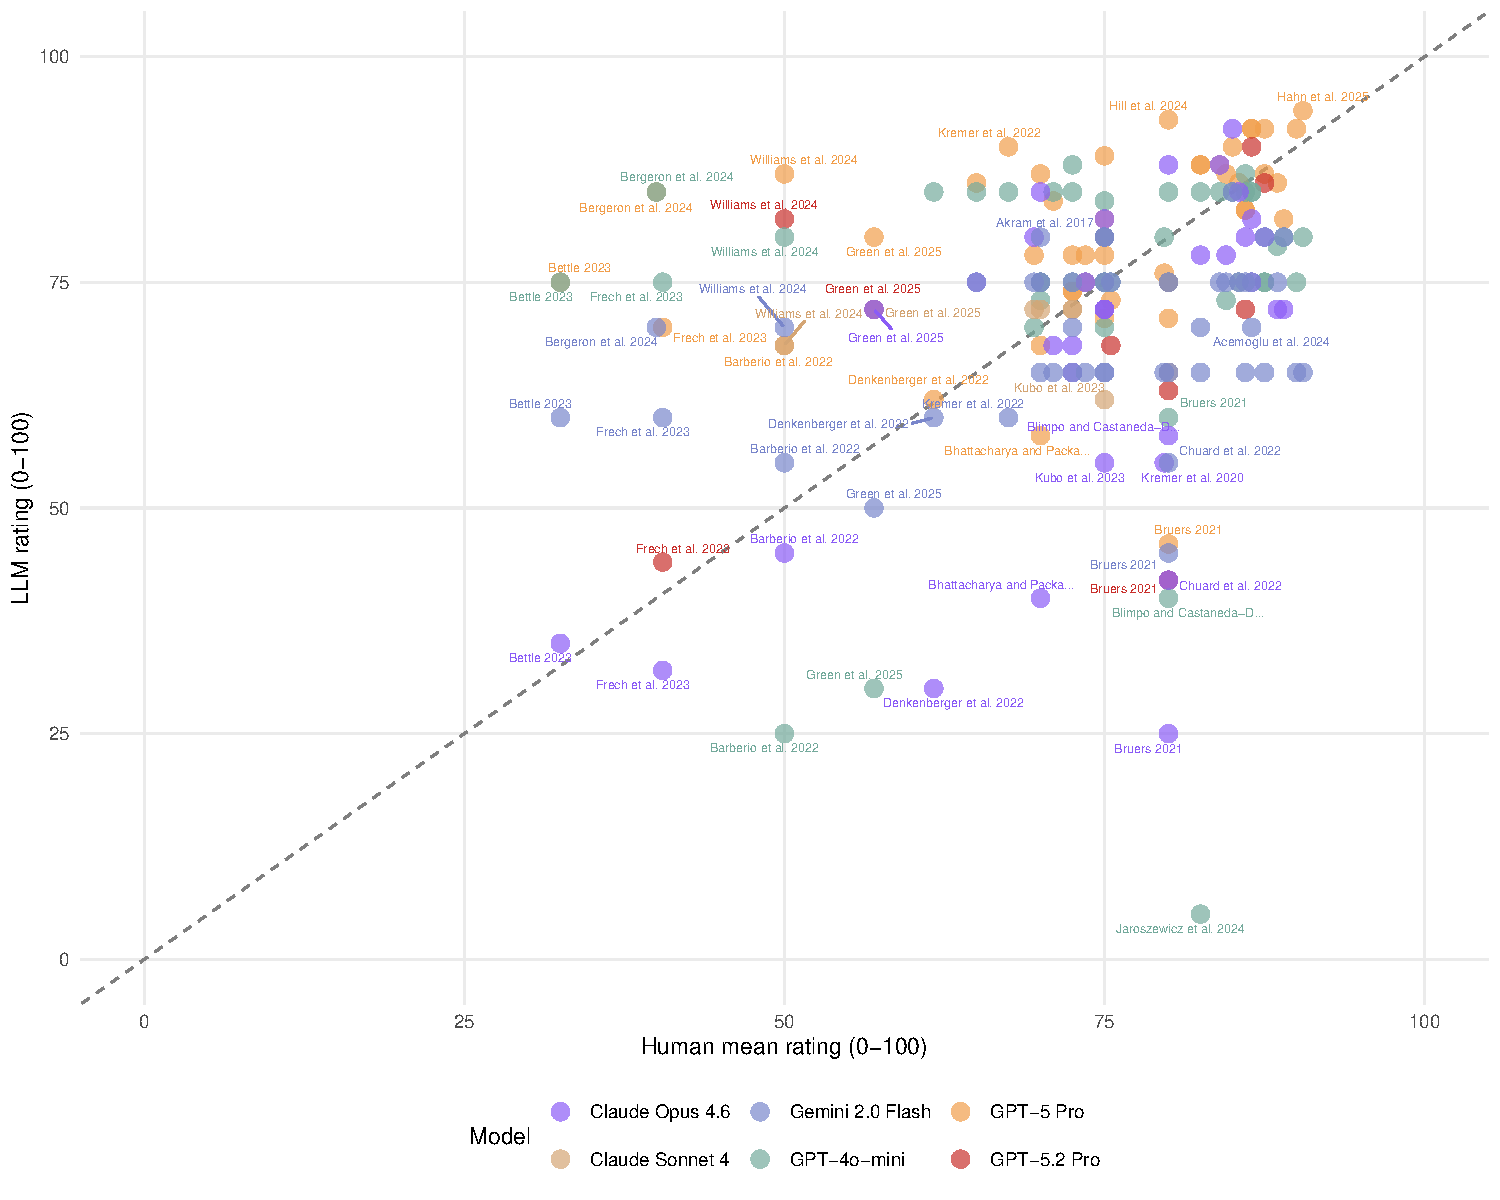
\includegraphics[keepaspectratio]{results_ratings_files/figure-pdf/fig-scatter-1.pdf}}

\end{figure}%

\section{Model Agreement Statistics}\label{model-agreement-statistics}

We assess agreement between LLM and human evaluators using multiple
metrics:

\begin{itemize}
\tightlist
\item
  \textbf{Pearson r}: Linear correlation between ratings
\item
  \textbf{Spearman ρ}: Rank-based correlation (robust to outliers)
\item
  \textbf{Mean bias}: Average difference (LLM − Human); positive = LLM
  rates higher
\item
  \textbf{RMSE/MAE}: Error magnitude measures
\end{itemize}

\begin{longtable}[]{@{}lrrrrrr@{}}

\caption{\label{tbl-agreement}Agreement between each LLM and human mean
ratings (overall criterion)}

\tabularnewline

\toprule\noalign{}
Model & N & Pearson r & Spearman ρ & Mean bias & RMSE & MAE \\
\midrule\noalign{}
\endhead
\bottomrule\noalign{}
\endlastfoot
Gemini 2.0 Flash & 44 & 0.351 & 0.321 & -5.0 & 14.4 & 11.6 \\
GPT-5 Pro & 45 & 0.342 & 0.517 & +6.4 & 15.4 & 10.3 \\
GPT-5.2 Pro & 9 & 0.333 & 0.471 & -2.7 & 19.0 & 14.7 \\
Claude Sonnet 4 & 10 & 0.197 & 0.272 & +1.5 & 9.1 & 6.3 \\
GPT-4o-mini & 45 & 0.135 & 0.116 & +0.0 & 20.2 & 13.1 \\

\end{longtable}

\subsection{Inter-Rater Agreement (Krippendorff's
Alpha)}\label{inter-rater-agreement-krippendorffs-alpha}

Krippendorff's alpha measures agreement among multiple raters,
accounting for chance agreement. Values above 0.8 indicate good
agreement; 0.67--0.8 is acceptable for exploratory research. Ceiling
effects apply because human evaluators are not perfectly aligned.

\begin{longtable}[]{@{}lrl@{}}

\caption{\label{tbl-krippendorff}Inter-rater agreement: Krippendorff's
alpha by criterion}

\tabularnewline

\toprule\noalign{}
Criterion & Krippendorff's α & Interpretation \\
\midrule\noalign{}
\endhead
\bottomrule\noalign{}
\endlastfoot
Overall & 0.221 & Poor \\
Claims & 0.335 & Poor \\
Methods & 0.192 & Poor \\
Adv. Knowledge & 0.144 & Poor \\
Logic \& Comms & 0.021 & Poor \\
Open Science & 0.093 & Poor \\
Global Relevance & 0.189 & Poor \\

\end{longtable}

\subsection[Human-Human vs Human-LLM Agreement (Baseline
Context)]{\texorpdfstring{Human-Human vs Human-LLM Agreement (Baseline
Context)\footnote{This section was added with AI assistance to address
  feedback about contextualizing agreement metrics.}}{Human-Human vs Human-LLM Agreement (Baseline Context)}}\label{human-human-vs-human-llm-agreement-baseline-contextresults_ratings-2}

To interpret human-LLM agreement, we must compare against
\textbf{human-human agreement} as an upper bound. If human evaluators
only agree with each other at α = 0.5, then expecting LLMs to achieve α
= 0.8 with humans would be unrealistic. The table below shows both:

\begin{itemize}
\tightlist
\item
  \textbf{α\textsubscript{HH}}: Krippendorff's alpha among human
  evaluators (treating each evaluator as a separate rater)
\item
  \textbf{α\textsubscript{HL}}: Krippendorff's alpha between human mean
  and each LLM model
\end{itemize}

\begin{longtable}[]{@{}
  >{\raggedright\arraybackslash}p{(\linewidth - 12\tabcolsep) * \real{0.1371}}
  >{\raggedleft\arraybackslash}p{(\linewidth - 12\tabcolsep) * \real{0.0403}}
  >{\raggedleft\arraybackslash}p{(\linewidth - 12\tabcolsep) * \real{0.1371}}
  >{\raggedleft\arraybackslash}p{(\linewidth - 12\tabcolsep) * \real{0.1532}}
  >{\raggedleft\arraybackslash}p{(\linewidth - 12\tabcolsep) * \real{0.1532}}
  >{\raggedleft\arraybackslash}p{(\linewidth - 12\tabcolsep) * \real{0.1855}}
  >{\raggedleft\arraybackslash}p{(\linewidth - 12\tabcolsep) * \real{0.1935}}@{}}

\caption{\label{tbl-human-baseline}Human-human vs Human-LLM agreement by
criterion (Krippendorff's α)}

\tabularnewline

\toprule\noalign{}
\begin{minipage}[b]{\linewidth}\raggedright
Criterion
\end{minipage} & \begin{minipage}[b]{\linewidth}\raggedleft
α\_HH
\end{minipage} & \begin{minipage}[b]{\linewidth}\raggedleft
α\_HL (GPT-5 Pro)
\end{minipage} & \begin{minipage}[b]{\linewidth}\raggedleft
α\_HL (GPT-5.2 Pro)
\end{minipage} & \begin{minipage}[b]{\linewidth}\raggedleft
α\_HL (GPT-4o-mini)
\end{minipage} & \begin{minipage}[b]{\linewidth}\raggedleft
α\_HL (Claude Sonnet 4)
\end{minipage} & \begin{minipage}[b]{\linewidth}\raggedleft
α\_HL (Gemini 2.0 Flash)
\end{minipage} \\
\midrule\noalign{}
\endhead
\bottomrule\noalign{}
\endlastfoot
Overall & 0.55 & 0.25 & 0.36 & 0.14 & 0.14 & 0.26 \\
Claims & 0.42 & 0.20 & 0.26 & 0.19 & 0.21 & 0.18 \\
Methods & 0.54 & 0.29 & 0.07 & 0.03 & -0.22 & 0.16 \\
Adv. Knowledge & 0.20 & 0.18 & 0.20 & 0.13 & 0.08 & 0.07 \\
Logic \& Comms & 0.33 & -0.04 & -0.19 & -0.00 & 0.25 & -0.05 \\
Open Science & 0.03 & -0.06 & -0.61 & -0.16 & 0.30 & 0.01 \\
Global Relevance & 0.33 & 0.25 & 0.51 & 0.04 & -0.20 & 0.18 \\

\end{longtable}

\textbf{Interpretation}: If α\textsubscript{HL} approaches or exceeds
α\textsubscript{HH}, the LLM is performing at or above the level of
agreement humans achieve with each other---a meaningful benchmark for
``human-level'' evaluation consistency.

\subsection[Uncertainty Interval Coverage (LLM Credible Interval
Assessment)]{\texorpdfstring{Uncertainty Interval Coverage (LLM Credible
Interval
Assessment)\footnote{This analysis addresses feedback about LLM
  uncertainty quantification.}}{Uncertainty Interval Coverage (LLM Credible Interval Assessment)}}\label{uncertainty-interval-coverage-llm-credible-interval-assessmentresults_ratings-3}

LLMs report 90\% credible intervals alongside their point estimates. If
these intervals are \textbf{well-specified}, approximately 90\% of human
mean ratings should fall within them. Lower coverage suggests the LLM is
overconfident; higher coverage suggests unnecessary uncertainty.

\begin{longtable}[]{@{}
  >{\raggedright\arraybackslash}p{(\linewidth - 10\tabcolsep) * \real{0.2024}}
  >{\raggedleft\arraybackslash}p{(\linewidth - 10\tabcolsep) * \real{0.1190}}
  >{\raggedleft\arraybackslash}p{(\linewidth - 10\tabcolsep) * \real{0.1429}}
  >{\raggedleft\arraybackslash}p{(\linewidth - 10\tabcolsep) * \real{0.1429}}
  >{\raggedleft\arraybackslash}p{(\linewidth - 10\tabcolsep) * \real{0.1905}}
  >{\raggedleft\arraybackslash}p{(\linewidth - 10\tabcolsep) * \real{0.2024}}@{}}

\caption{\label{tbl-ci-coverage}Share of human mean ratings within LLM
90\% credible intervals}

\tabularnewline

\toprule\noalign{}
\begin{minipage}[b]{\linewidth}\raggedright
Criterion
\end{minipage} & \begin{minipage}[b]{\linewidth}\raggedleft
GPT-5 Pro
\end{minipage} & \begin{minipage}[b]{\linewidth}\raggedleft
GPT-5.2 Pro
\end{minipage} & \begin{minipage}[b]{\linewidth}\raggedleft
GPT-4o-mini
\end{minipage} & \begin{minipage}[b]{\linewidth}\raggedleft
Claude Sonnet 4
\end{minipage} & \begin{minipage}[b]{\linewidth}\raggedleft
Gemini 2.0 Flash
\end{minipage} \\
\midrule\noalign{}
\endhead
\bottomrule\noalign{}
\endlastfoot
Overall & 64\% & 44\% & 49\% & 70\% & 66\% \\
Claims & 39\% & 44\% & 44\% & 43\% & 56\% \\
Methods & 59\% & 22\% & 55\% & 40\% & 60\% \\
Adv. Knowledge & 55\% & 44\% & 52\% & 60\% & 65\% \\
Logic \& Comms & 36\% & 44\% & 62\% & 50\% & 68\% \\
Open Science & 33\% & 33\% & 40\% & 60\% & 48\% \\
Global Relevance & 49\% & 89\% & 44\% & 60\% & 59\% \\

\end{longtable}

\textbf{Interpretation}: Coverage near 90\% indicates well-specified
uncertainty. Coverage below 70\% suggests systematic overconfidence;
coverage above 95\% may indicate overly wide intervals that provide
little information.

\subsection[Statistical Significance of Agreement
Measures]{\texorpdfstring{Statistical Significance of Agreement
Measures\footnote{Bootstrap inference was added with AI assistance to
  quantify uncertainty in agreement metrics.}}{Statistical Significance of Agreement Measures}}\label{statistical-significance-of-agreement-measuresresults_ratings-4}

To assess whether observed correlations are statistically meaningful and
to compare models, we compute \textbf{bootstrap 95\% confidence
intervals} for Pearson correlations. This nonparametric approach makes
no distributional assumptions and accounts for the small sample sizes
typical in evaluation studies.

\begin{longtable}[]{@{}lrrr@{}}

\caption{\label{tbl-bootstrap-ci}Bootstrap 95\% CIs for human-LLM
correlation (overall ratings)}

\tabularnewline

\toprule\noalign{}
Model & n & r & 95\% CI \\
\midrule\noalign{}
\endhead
\bottomrule\noalign{}
\endlastfoot
Gemini 2.0 Flash & 44 & 0.35 & {[}0.10, 0.56{]} \\
GPT-5 Pro & 45 & 0.34 & {[}0.09, 0.59{]} \\
GPT-5.2 Pro & 9 & 0.33 & {[}-0.47, 0.88{]} \\
Claude Sonnet 4 & 10 & 0.20 & {[}-0.66, 0.94{]} \\
GPT-4o-mini & 45 & 0.13 & {[}-0.15, 0.46{]} \\

\end{longtable}

\textbf{Interpretation}: Non-overlapping confidence intervals suggest
statistically distinguishable performance. Wide intervals reflect
uncertainty due to limited sample size---a common constraint in
evaluation research where obtaining more human judgments is costly.

\subsection[Information-Theoretic Perspective: Mutual
Information]{\texorpdfstring{Information-Theoretic Perspective: Mutual
Information\footnote{Information-theoretic interpretation added with AI
  assistance.}}{Information-Theoretic Perspective: Mutual Information}}\label{information-theoretic-perspective-mutual-informationresults_ratings-5}

Beyond correlation, we can ask: \textbf{how much information do LLM
ratings convey about human ratings?} We use \emph{mutual information}
(MI), a fundamental concept from information theory
(\citeproc{ref-shannon1948mathematical}{Shannon 1948};
\citeproc{ref-cover2006elements}{Cover and Thomas 2006}).

\textbf{What is mutual information?} MI quantifies the \emph{reduction
in uncertainty} about one variable when you learn the value of another.
Formally, MI(X;Y) = H(X) - H(X\textbar Y), where H is entropy (average
surprise/uncertainty). In plain terms:

\begin{itemize}
\tightlist
\item
  Before seeing the LLM rating, you have some uncertainty about what the
  human rating will be
\item
  After seeing the LLM rating, how much does your uncertainty decrease?
\item
  MI measures this decrease, in \emph{bits} (the same unit used in data
  compression and communication)
\end{itemize}

\textbf{Why use MI instead of (or alongside) correlation?}

\begin{longtable}[]{@{}
  >{\raggedright\arraybackslash}p{(\linewidth - 4\tabcolsep) * \real{0.4789}}
  >{\raggedright\arraybackslash}p{(\linewidth - 4\tabcolsep) * \real{0.2394}}
  >{\raggedright\arraybackslash}p{(\linewidth - 4\tabcolsep) * \real{0.2817}}@{}}
\toprule\noalign{}
\begin{minipage}[b]{\linewidth}\raggedright
Property
\end{minipage} & \begin{minipage}[b]{\linewidth}\raggedright
Correlation (r)
\end{minipage} & \begin{minipage}[b]{\linewidth}\raggedright
Mutual Information
\end{minipage} \\
\midrule\noalign{}
\endhead
\bottomrule\noalign{}
\endlastfoot
Captures linear relationships & Yes & Yes \\
Captures nonlinear relationships & No & Yes \\
Detects threshold effects & No & Yes \\
Scale & -1 to +1 & 0 to ∞ bits \\
Sensitive to outliers & Yes & Less so \\
\end{longtable}

A practical example: suppose the LLM predicts human ratings perfectly
when the paper is methodology-focused, but randomly when it's
theory-focused. Correlation might show r = 0.5 (moderate), but MI would
reveal this is \emph{inconsistent} performance rather than
\emph{uniformly moderate} performance. This distinction matters for
deciding when to trust LLM evaluations.

\textbf{How to interpret MI values (for 5-bin discretization):}

\begin{itemize}
\tightlist
\item
  \textbf{0 bits}: Independence---LLM ratings tell you nothing about
  human ratings
\item
  \textbf{\textasciitilde0.5 bits}: Weak association---knowing LLM
  rating slightly reduces uncertainty
\item
  \textbf{\textasciitilde1.0 bits}: Moderate association---knowing LLM
  rating roughly halves your uncertainty
\item
  \textbf{\textasciitilde1.5 bits}: Strong association---substantial
  predictive value
\item
  \textbf{2.32 bits} (maximum): Perfect prediction---the LLM quintile
  perfectly determines the human quintile
\end{itemize}

We discretize ratings into quintiles (5 bins) because MI is formally
defined for discrete distributions. This preserves ordinal structure
while avoiding overfitting to noise in continuous ratings.

\begin{longtable}[]{@{}lrrr@{}}

\caption{\label{tbl-mutual-info}Mutual information between human and LLM
overall ratings}

\tabularnewline

\toprule\noalign{}
Model & n & MI (bits) & Normalized \\
\midrule\noalign{}
\endhead
\bottomrule\noalign{}
\endlastfoot
GPT-5 Pro & 45 & 0.60 & 26\% \\
GPT-5.2 Pro & 9 & 1.61 & 70\% \\
GPT-4o-mini & 45 & 0.30 & 13\% \\
Claude Sonnet 4 & 10 & 0.77 & 33\% \\
Gemini 2.0 Flash & 44 & 0.14 & 6\% \\

\end{longtable}

\textbf{Interpretation}: Normalized MI above 50\% indicates substantial
predictive value. If MI is low despite moderate correlation, investigate
which paper characteristics the LLM struggles with---this points toward
targeted improvements or hybrid human-AI workflows where humans handle
cases the LLM finds difficult.

\subsection{Agreement by Evaluation
Criterion}\label{agreement-by-evaluation-criterion}

\begin{longtable}[]{@{}
  >{\raggedright\arraybackslash}p{(\linewidth - 10\tabcolsep) * \real{0.1889}}
  >{\raggedleft\arraybackslash}p{(\linewidth - 10\tabcolsep) * \real{0.1778}}
  >{\raggedleft\arraybackslash}p{(\linewidth - 10\tabcolsep) * \real{0.1556}}
  >{\raggedleft\arraybackslash}p{(\linewidth - 10\tabcolsep) * \real{0.1333}}
  >{\raggedleft\arraybackslash}p{(\linewidth - 10\tabcolsep) * \real{0.1556}}
  >{\raggedleft\arraybackslash}p{(\linewidth - 10\tabcolsep) * \real{0.1889}}@{}}

\caption{\label{tbl-agreement-by-criterion}Pearson and Spearman
correlations by evaluation criterion}

\tabularnewline

\toprule\noalign{}
\begin{minipage}[b]{\linewidth}\raggedright
Criterion
\end{minipage} & \begin{minipage}[b]{\linewidth}\raggedleft
Claude Sonnet 4
\end{minipage} & \begin{minipage}[b]{\linewidth}\raggedleft
GPT-4o-mini
\end{minipage} & \begin{minipage}[b]{\linewidth}\raggedleft
GPT-5 Pro
\end{minipage} & \begin{minipage}[b]{\linewidth}\raggedleft
GPT-5.2 Pro
\end{minipage} & \begin{minipage}[b]{\linewidth}\raggedleft
Gemini 2.0 Flash
\end{minipage} \\
\midrule\noalign{}
\endhead
\bottomrule\noalign{}
\endlastfoot
Overall & 0.20 / 0.27 & 0.13 / 0.12 & 0.34 / 0.52 & 0.33 / 0.47 & 0.35 /
0.32 \\
Claims & 0.46 / 0.28 & 0.18 / 0.28 & 0.21 / 0.39 & 0.25 / 0.32 & 0.21 /
0.05 \\
Methods & -0.47 / -0.61 & 0.03 / 0.12 & 0.34 / 0.54 & 0.02 / 0.05 & 0.19
/ 0.19 \\
Adv. Knowledge & 0.17 / 0.23 & 0.12 / 0.04 & 0.30 / 0.46 & 0.16 / 0.15 &
0.10 / 0.10 \\
Logic \& Comms & 0.52 / 0.56 & -0.01 / -0.02 & 0.19 / 0.28 & -0.25 /
-0.27 & 0.07 / 0.08 \\
Open Science & 0.29 / 0.44 & -0.13 / -0.13 & 0.17 / 0.12 & -0.60 / -0.51
& -0.00 / -0.09 \\
Global Relevance & -0.25 / -0.21 & 0.03 / 0.09 & 0.35 / 0.43 & 0.50 /
0.36 & 0.23 / 0.20 \\

\end{longtable}

\section{Criteria-Level Comparison}\label{criteria-level-comparison}

\begin{figure}

\caption{\label{fig-criteria-heatmap}Mean rating by model and criterion}

\pandocbounded{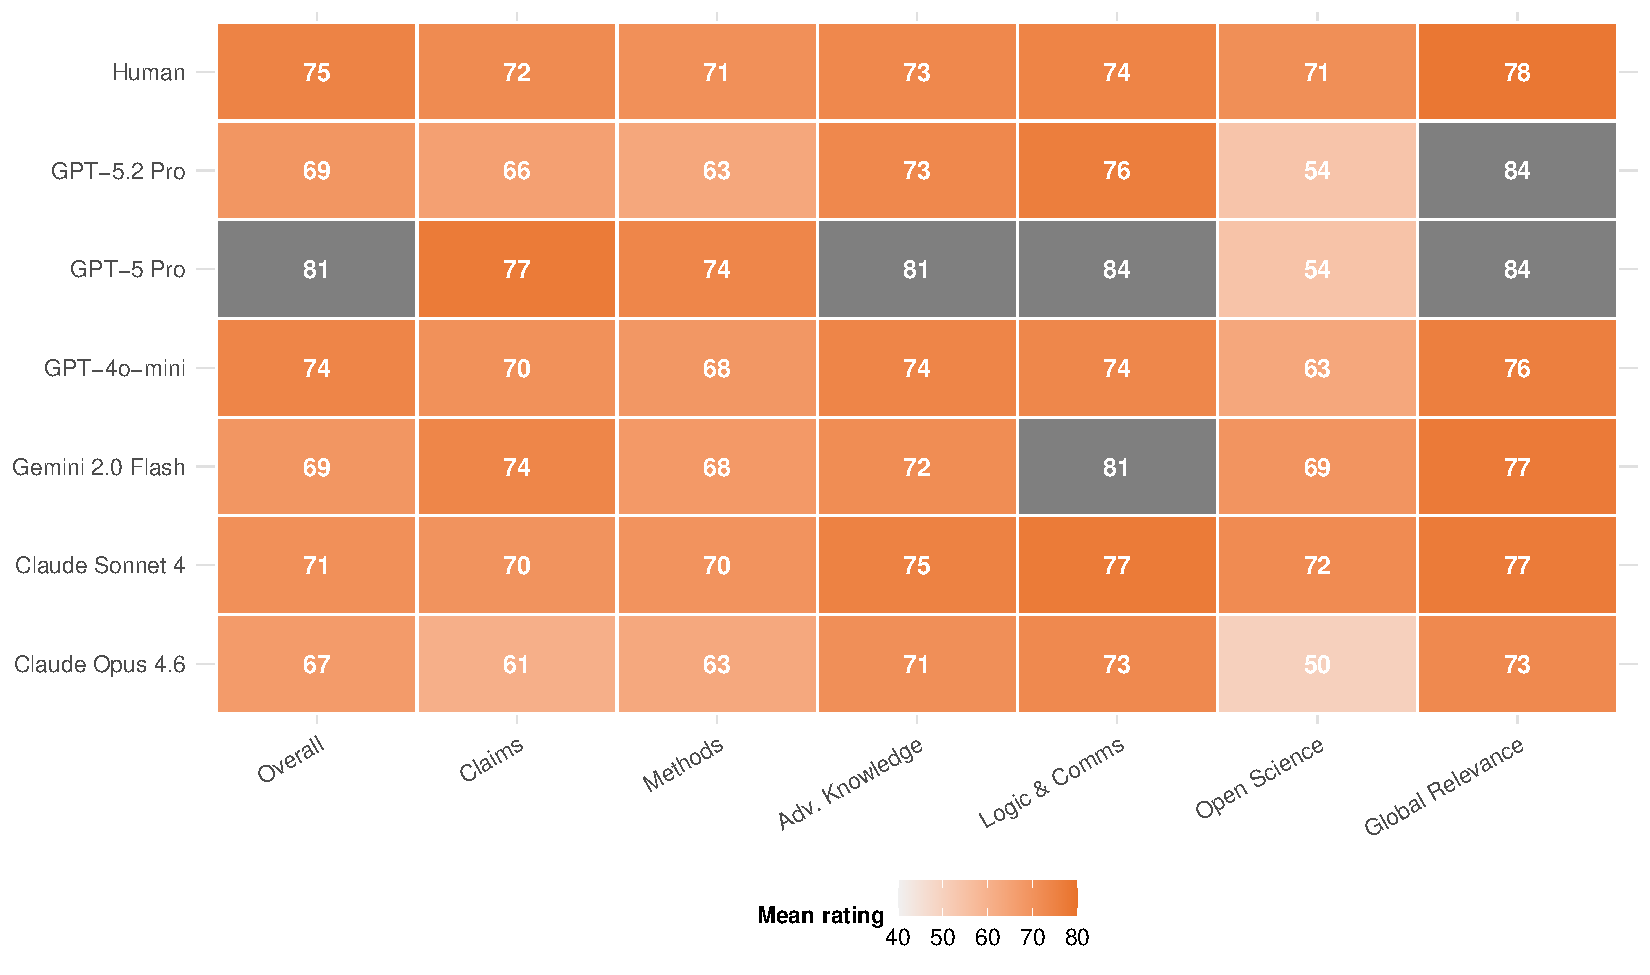
\includegraphics[keepaspectratio]{results_ratings_files/figure-pdf/fig-criteria-heatmap-1.pdf}}

\end{figure}%

\section[Evaluation Priorities: What Predicts Journal Tier
Judgments?]{\texorpdfstring{Evaluation Priorities: What Predicts Journal
Tier
Judgments?\footnote{This analysis was added with AI assistance to reveal
  differences in what humans vs.~LLMs emphasize when predicting journal
  outcomes.}}{Evaluation Priorities: What Predicts Journal Tier Judgments?}}\label{evaluation-priorities-what-predicts-journal-tier-judgmentsresults_ratings-6}

How do evaluators translate quality assessments into journal tier
predictions? By correlating each criterion with ``where should this
publish?'' judgments, we can see which factors each evaluator type
weighs most heavily. Divergence here reveals systematic differences in
evaluation priorities---what we might call ``taste.''

\begin{verbatim}
Tier prediction column not found in human data.
\end{verbatim}

\textbf{Interpretation}: Large divergences indicate different evaluation
philosophies. For example, if humans weight ``open science'' heavily but
LLMs don't, this suggests the LLM may undervalue reproducibility when
forming overall judgments.

\begin{center}\rule{0.5\linewidth}{0.5pt}\end{center}

\section[Systematic Rating Differences by Paper and
Criterion]{\texorpdfstring{Systematic Rating Differences by Paper and
Criterion\footnote{This visualization was added with AI assistance to
  identify patterns in human-LLM disagreement.}}{Systematic Rating Differences by Paper and Criterion}}\label{systematic-rating-differences-by-paper-and-criterionresults_ratings-7}

The heatmap below shows \textbf{Human − LLM} differences for each paper
and criterion. Green indicates humans rated higher than the LLM; orange
indicates the LLM rated higher. Papers are ordered by their overall
rating difference.

\begin{figure}

\caption{\label{fig-gap-heatmap}Human − LLM rating differences by paper
and criterion}

\pandocbounded{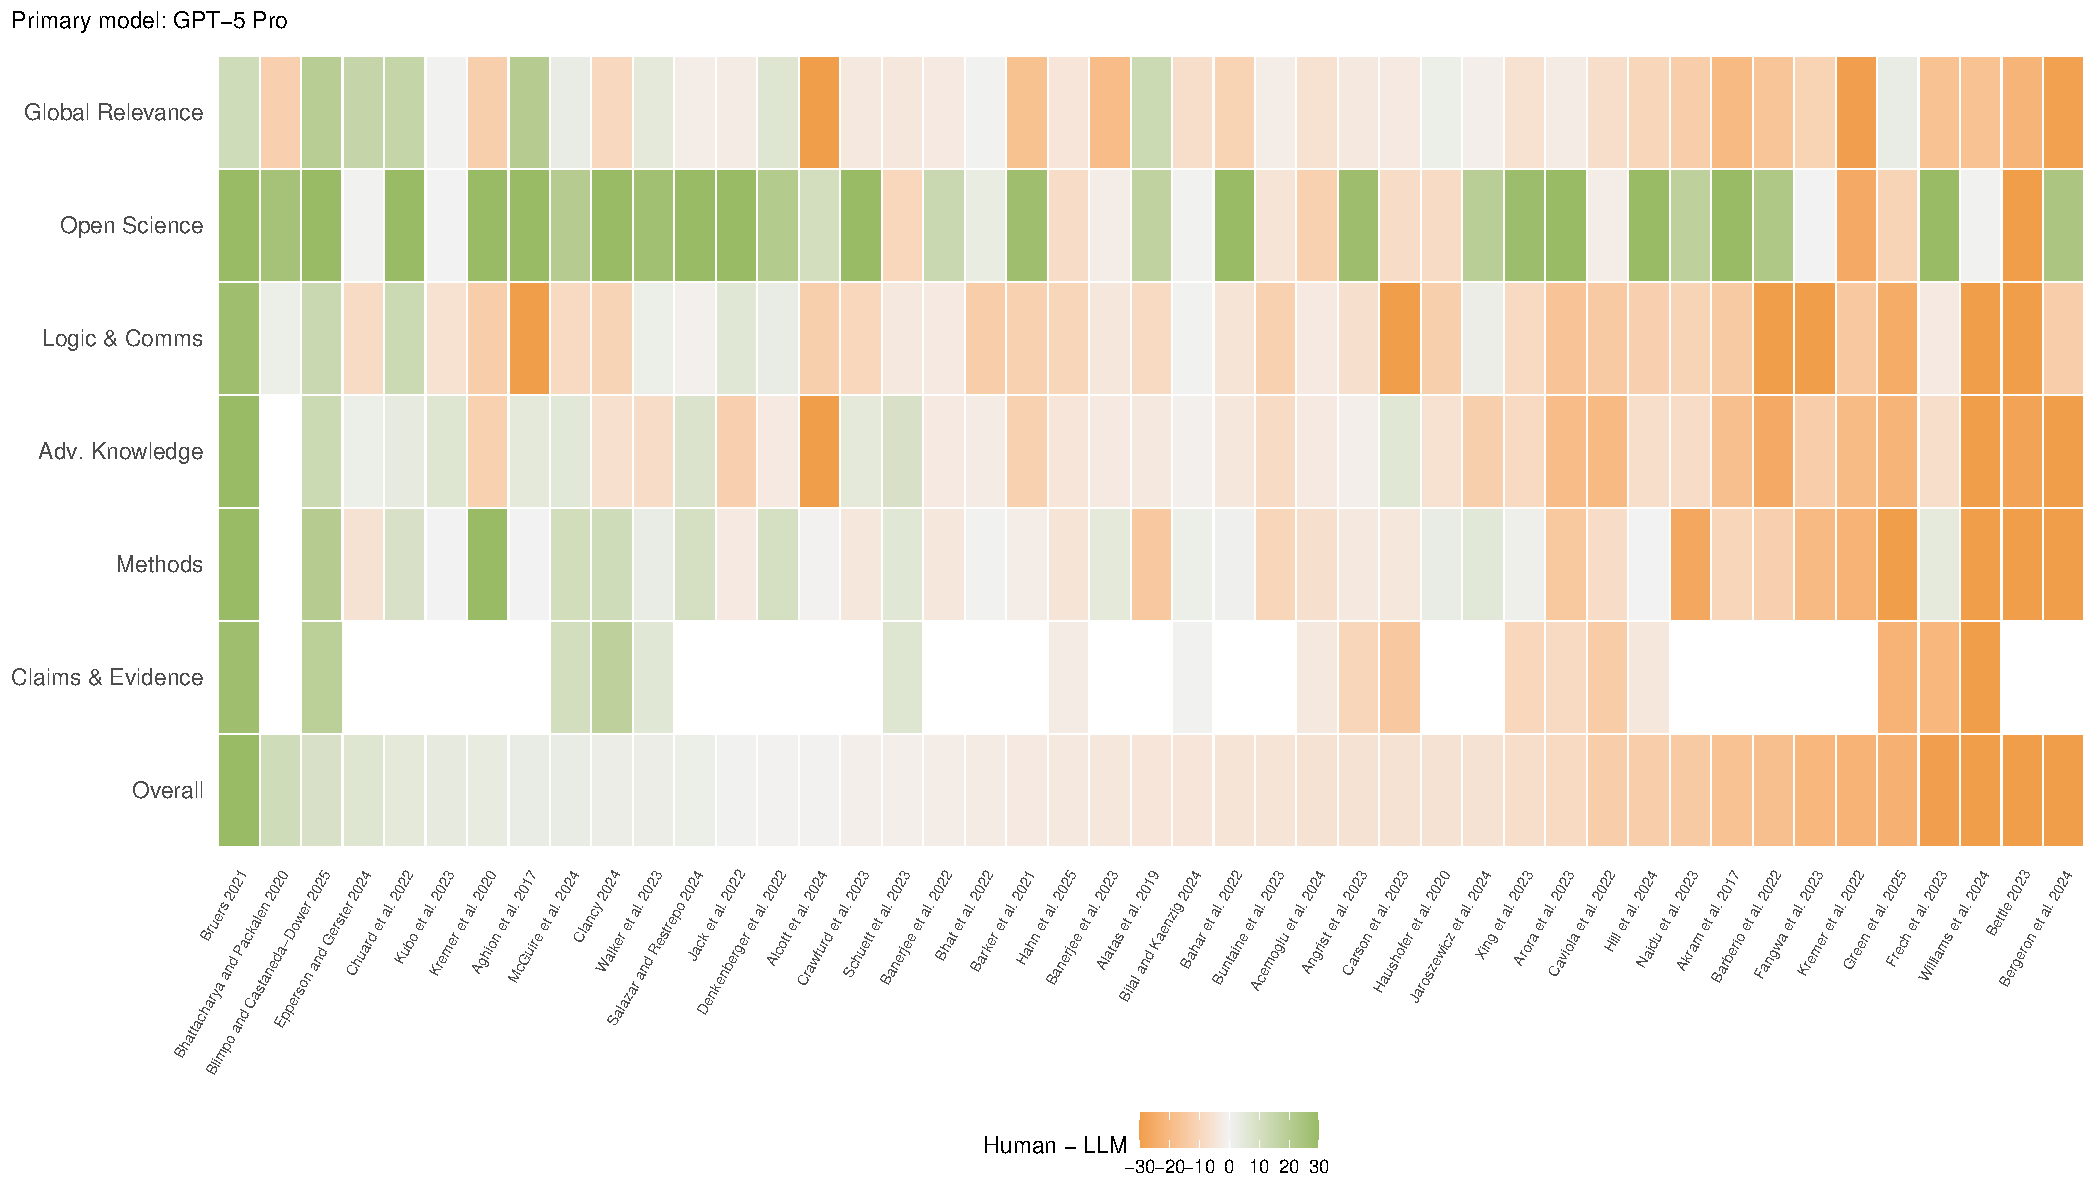
\includegraphics[keepaspectratio]{results_ratings_files/figure-pdf/fig-gap-heatmap-1.pdf}}

\end{figure}%

This visualization helps identify: (1) papers with systematic
disagreement across all criteria, (2) criteria where humans and LLMs
consistently diverge, and (3) potential patterns related to paper
characteristics.

\section[Papers with Largest Human-LLM
Disagreement]{\texorpdfstring{Papers with Largest Human-LLM
Disagreement\footnote{This table was added with AI assistance to
  facilitate qualitative investigation of outliers.}}{Papers with Largest Human-LLM Disagreement}}\label{papers-with-largest-human-llm-disagreementresults_ratings-8}

Understanding \emph{why} specific papers generate disagreement can
inform both LLM limitations and potential human biases. The table below
shows papers where humans and LLMs diverged most.

\begin{longtable}[]{@{}
  >{\raggedright\arraybackslash}p{(\linewidth - 8\tabcolsep) * \real{0.4051}}
  >{\raggedleft\arraybackslash}p{(\linewidth - 8\tabcolsep) * \real{0.1646}}
  >{\raggedleft\arraybackslash}p{(\linewidth - 8\tabcolsep) * \real{0.1392}}
  >{\raggedleft\arraybackslash}p{(\linewidth - 8\tabcolsep) * \real{0.1392}}
  >{\raggedright\arraybackslash}p{(\linewidth - 8\tabcolsep) * \real{0.1519}}@{}}

\caption{\label{tbl-top-disagreement}Papers with largest human vs.~LLM
rating differences}

\tabularnewline

\toprule\noalign{}
\begin{minipage}[b]{\linewidth}\raggedright
Paper
\end{minipage} & \begin{minipage}[b]{\linewidth}\raggedleft
Human Rating
\end{minipage} & \begin{minipage}[b]{\linewidth}\raggedleft
LLM Rating
\end{minipage} & \begin{minipage}[b]{\linewidth}\raggedleft
Difference
\end{minipage} & \begin{minipage}[b]{\linewidth}\raggedright
Direction
\end{minipage} \\
\midrule\noalign{}
\endhead
\bottomrule\noalign{}
\endlastfoot
Bruers 2021 & 80 & 46 & +34 & Human \textgreater{} LLM \\
Bhattacharya and Packalen 2020 & 70 & 58 & +12 & Human \textgreater{}
LLM \\
Blimpo and Castaneda-Dower 2025 & 80 & 71 & +9 & Human \textgreater{}
LLM \\
Epperson and Gerster 2024 & 89 & 82 & +7 & Human \textgreater{} LLM \\
Chuard et al.~2022 & 80 & 75 & +5 & Human \textgreater{} LLM \\
Bergeron et al.~2024 & 40 & 85 & -45 & LLM \textgreater{} Human \\
Bettle 2023 & 32 & 75 & -42 & LLM \textgreater{} Human \\
Williams et al.~2024 & 50 & 87 & -37 & LLM \textgreater{} Human \\
Frech et al.~2023 & 40 & 70 & -30 & LLM \textgreater{} Human \\
Green et al.~2025 & 57 & 80 & -23 & LLM \textgreater{} Human \\

\end{longtable}

These outliers merit qualitative investigation: examining the paper
characteristics, human evaluator comments, and LLM rationales may reveal
systematic patterns in what drives disagreement.

\begin{center}\rule{0.5\linewidth}{0.5pt}\end{center}

\emph{Note: GPT-5 Pro evaluations include extended reasoning traces. See
the \href{appendix_llm_traces.qmd}{Appendix} for full assessment
summaries and reasoning traces per paper.}

\section{Prompt Comparison: Legacy vs Updated GPT-5
Pro}\label{prompt-comparison-legacy-vs-updated-gpt-5-pro}

We compare GPT-5 Pro evaluations between two prompt versions:

\begin{itemize}
\tightlist
\item
  \textbf{Legacy (Oct 2024):} Original combined schema without
  assessment summary
\item
  \textbf{Updated (Jan 2026):} Modular prompt with explicit diagnostic
  assessment summary
\end{itemize}

We matched 57 papers across both runs.

\begin{longtable}[t]{lrrrr}

\caption{\label{tbl-prompt-summary}Summary statistics: Legacy vs Updated
prompt}

\tabularnewline

\toprule
Criterion & Legacy Mean & Updated Mean & Mean Diff & SD Diff\\
\midrule
Adv. Knowledge & 84.5 & 80.4 & -4.1 & 4.8\\
Claims & 83.2 & 77.5 & -5.7 & 4.8\\
Global Relevance & 85.8 & 82.6 & -3.2 & 6.3\\
Logic \& Comms & 86.4 & 83.6 & -2.8 & 4.8\\
Methods & 81.3 & 73.6 & -7.7 & 4.6\\
\addlinespace
Open Science & 67.9 & 54.8 & -13.1 & 8.9\\
Overall & 86.0 & 80.4 & -5.6 & 4.4\\
\bottomrule

\end{longtable}

The updated prompt with explicit diagnostic assessment appears to
produce systematically different ratings. The summary table above
quantifies the shift; scatter and boxplot visualizations of the prompt
comparison are available in the full online version.

\bookmarksetup{startatroot}

\chapter{Results: Critiques \& Key
Issues}\label{results-critiques-key-issues}

This chapter compares \emph{qualitative critiques}: the key
methodological and interpretive issues identified by the LLM model ---
against human expert critiques documented by Unjournal evaluation
managers in Coda.

We first assess alignment using LLM-based comparison: GPT-5.2 Pro
evaluates coverage (what proportion of human concerns GPT identified)
and precision (whether GPT issues are substantive). Human-checks on this
alignment are underway. See \hyperref[sec-llm-assessment]{LLM-Based
Assessment} for aggregate metrics.

\section{Data Sources}\label{data-sources}

\textbf{GPT-5.2 Pro Key Issues}: Structured output from the focal
evaluation run (January 2026), where the model was prompted to identify
5-15 key issues per paper, ordered from most to least important.

\textbf{Human Expert Critiques}: Curated content from the ``Key
critiques \& issues with paper'' column in The Unjournal's internal
tracking database (Coda), written by evaluation managers synthesizing
evaluator feedback. These use severity labels (``Necessary'', ``Optional
but important'', ``Unsure'') and cite specific evaluator comments.

We matched \textbf{14 papers} with both GPT-5.2 Pro key issues and human
expert critiques.

\section{Overview Statistics}\label{overview-statistics}

\begin{longtable}[]{@{}lr@{}}

\caption{\label{tbl-overview-stats}Summary of key issues comparison
data}

\tabularnewline

\toprule\noalign{}
Metric & Value \\
\midrule\noalign{}
\endhead
\bottomrule\noalign{}
\endlastfoot
Papers Compared & 14.0 \\
Avg GPT Issues per Paper & 11.6 \\
Min GPT Issues & 10.0 \\
Max GPT Issues & 12.0 \\
Avg Coda Critique Length (chars) & 2311.0 \\
Min Coda Length & 1197.0 \\
Max Coda Length & 4998.0 \\

\end{longtable}

\section{Paper-by-Paper Comparison}\label{sec-paper-comparison}

Paper-by-paper comparisons with interactive collapsible panels are
available in the
\href{https://llm-uj-research-eval.netlify.app/results_critiques.html\#sec-paper-comparison}{online
HTML version}.

\section{LLM-Based Assessment}\label{sec-llm-assessment}

The comparison between GPT key issues and human critiques was assessed
using GPT-5.2 Pro, which evaluated coverage (what proportion of human
concerns GPT identified) and precision (whether GPT issues are
substantive).

\begin{itemize}
\tightlist
\item
  \textbf{Coverage}: Proportion of \emph{consensus} human issues that
  have any LLM match (match quality ≥ 30\%)
\item
  \textbf{Weighted Coverage}: Mean match quality across all human issues
  (treating unmatched issues as 0\%)
\item
  \textbf{Precision}: Proportion of LLM issues that match a human
  concern
\end{itemize}

\textbf{Note}: Any interpretation or narrative commentary in this
section is written by an LLM (Codex). The values themselves come from
the GPT-5.2 Pro comparison outputs.

\begin{tcolorbox}[enhanced jigsaw, colback=white, title=\textcolor{quarto-callout-note-color}{\faInfo}\hspace{0.5em}{Caveat on Precision}, bottomrule=.15mm, coltitle=black, left=2mm, colframe=quarto-callout-note-color-frame, toptitle=1mm, toprule=.15mm, titlerule=0mm, breakable, leftrule=.75mm, colbacktitle=quarto-callout-note-color!10!white, bottomtitle=1mm, arc=.35mm, rightrule=.15mm, opacityback=0, opacitybacktitle=0.6]

``Precision'' only reflects whether LLM issues match the
\emph{consensus} human issues curated in Coda---those prioritized by
evaluation managers as the most important concerns. Many LLM-identified
issues may have been noted by one or more individual human evaluators
but were not included in this curated set. A low precision score does
not necessarily mean the LLM raised irrelevant concerns; it may simply
reflect issues that weren't prioritized in the consensus summary.

\end{tcolorbox}

\begin{longtable}[]{@{}lr@{}}
\caption{LLM assessment of GPT vs human critique
alignment}\tabularnewline
\toprule\noalign{}
Metric & Value \\
\midrule\noalign{}
\endfirsthead
\toprule\noalign{}
Metric & Value \\
\midrule\noalign{}
\endhead
\bottomrule\noalign{}
\endlastfoot
Papers Assessed & 14 \\
Mean Coverage (\%) & 74.9 \\
Mean Precision (\%) & 46.9 \\
Coverage Range & 40-100 \\
Precision Range & 17-83 \\
\end{longtable}

\begin{figure}

\caption{\label{fig-coverage-precision}Coverage vs Precision across
papers (LLM-assessed)}

\pandocbounded{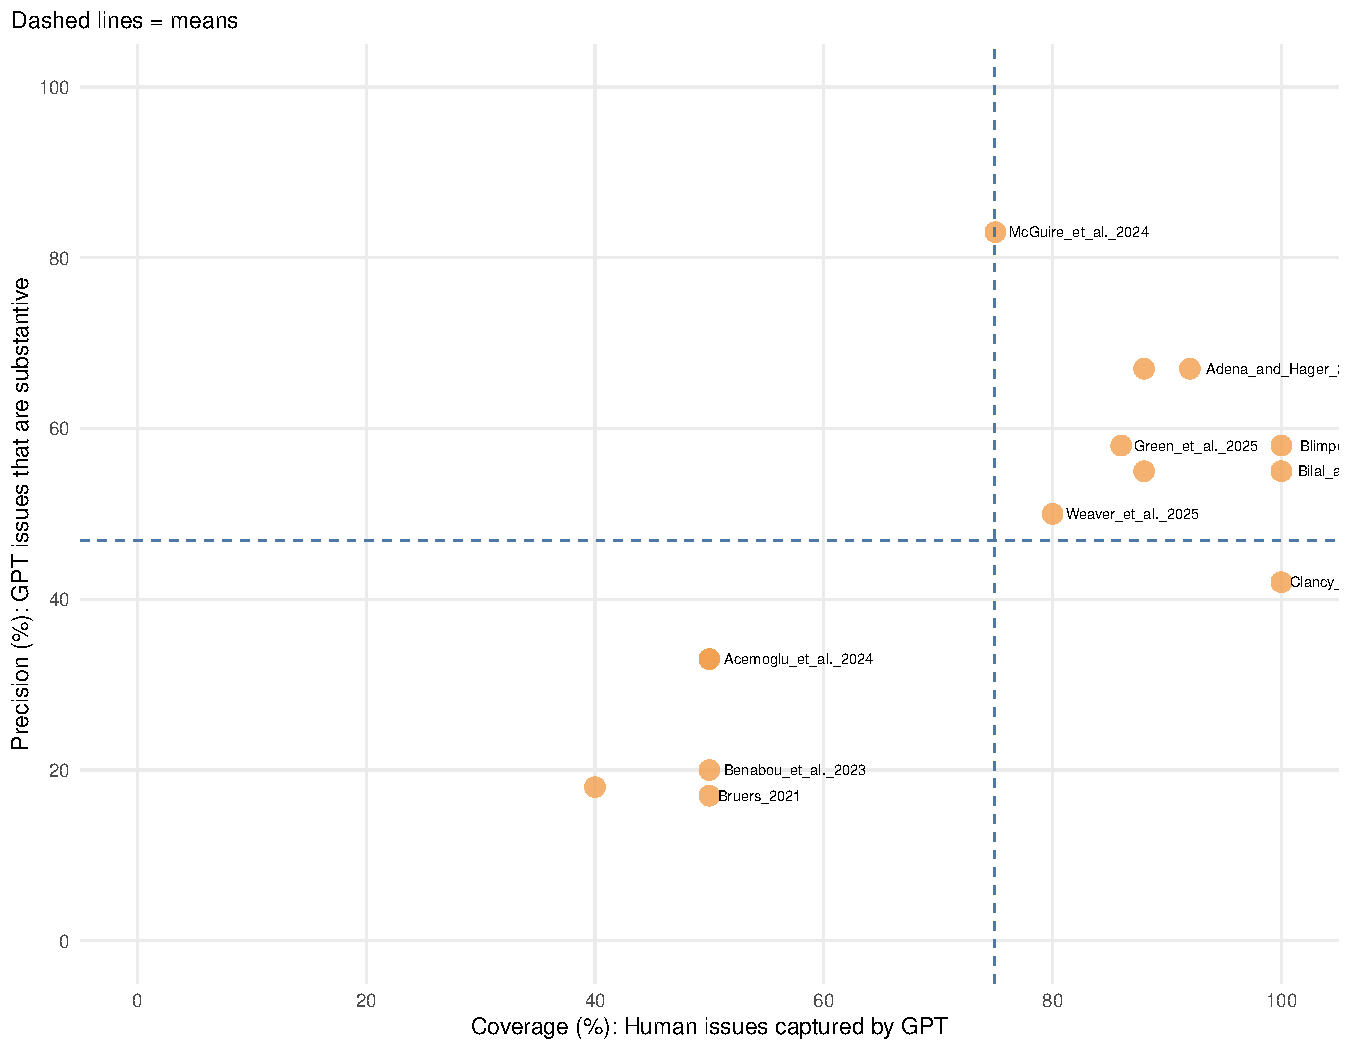
\includegraphics[keepaspectratio]{results_critiques_files/figure-pdf/fig-coverage-precision-1.pdf}}

\end{figure}%

\begin{longtable}[]{@{}
  >{\raggedright\arraybackslash}p{(\linewidth - 6\tabcolsep) * \real{0.4706}}
  >{\raggedleft\arraybackslash}p{(\linewidth - 6\tabcolsep) * \real{0.1912}}
  >{\raggedleft\arraybackslash}p{(\linewidth - 6\tabcolsep) * \real{0.2059}}
  >{\raggedright\arraybackslash}p{(\linewidth - 6\tabcolsep) * \real{0.1324}}@{}}

\caption{\label{tbl-paper-ratings}Per-paper LLM assessment results}

\tabularnewline

\toprule\noalign{}
\begin{minipage}[b]{\linewidth}\raggedright
Paper
\end{minipage} & \begin{minipage}[b]{\linewidth}\raggedleft
Coverage (\%)
\end{minipage} & \begin{minipage}[b]{\linewidth}\raggedleft
Precision (\%)
\end{minipage} & \begin{minipage}[b]{\linewidth}\raggedright
Rating
\end{minipage} \\
\midrule\noalign{}
\endhead
\bottomrule\noalign{}
\endlastfoot
Bilal\_and\_Kaenzig\_2024 & 100 & 55 & Good \\
Blimpo\_and\_Castaneda-Dower\_2025 & 100 & 58 & Good \\
Clancy\_2024 & 100 & 42 & Good \\
Adena\_and\_Hager\_2024 & 92 & 67 & Good \\
Dullaghan\_and\_Zhang\_2022 & 88 & 55 & Good \\
Williams\_et\_al.\_2024 & 88 & 67 & Good \\
Green\_et\_al.\_2025 & 86 & 58 & Good \\
Weaver\_et\_al.\_2025 & 80 & 50 & Moderate \\
McGuire\_et\_al.\_2024 & 75 & 83 & Good \\
Acemoglu\_et\_al.\_2024 & 50 & 33 & Moderate \\
Benabou\_et\_al.\_2023 & 50 & 20 & Poor \\
Bruers\_2021 & 50 & 17 & Moderate \\
Frech\_et\_al.\_2023 & 50 & 33 & Moderate \\
Peterman\_et\_al.\_2025 & 40 & 18 & Poor \\

\end{longtable}

\begin{tcolorbox}[enhanced jigsaw, colback=white, title=\textcolor{quarto-callout-note-color}{\faInfo}\hspace{0.5em}{Interpretation Guide}, bottomrule=.15mm, coltitle=black, left=2mm, colframe=quarto-callout-note-color-frame, toptitle=1mm, toprule=.15mm, titlerule=0mm, breakable, leftrule=.75mm, colbacktitle=quarto-callout-note-color!10!white, bottomtitle=1mm, arc=.35mm, rightrule=.15mm, opacityback=0, opacitybacktitle=0.6]

\begin{itemize}
\tightlist
\item
  \textbf{Coverage}: Percentage of human-identified issues that GPT also
  captured (in some form). Higher = GPT missed fewer human concerns.
\item
  \textbf{Precision}: Percentage of GPT issues that are substantive
  rather than generic or spurious. Higher = GPT's critiques are more
  targeted.
\item
  \textbf{Overall Rating}: Qualitative assessment
  (Excellent/Good/Moderate/Poor) based on both coverage and precision
  metrics.
\end{itemize}

\end{tcolorbox}

\section{Summary and Observations}\label{summary-and-observations}

\subsection{Aggregate Statistics}\label{aggregate-statistics}

\begin{longtable}[]{@{}lr@{}}
\caption{Aggregate statistics across all
papers}\label{tbl-aggregate-stats}\tabularnewline
\toprule\noalign{}
Metric & Value \\
\midrule\noalign{}
\endfirsthead
\toprule\noalign{}
Metric & Value \\
\midrule\noalign{}
\endhead
\bottomrule\noalign{}
\endlastfoot
Papers Compared & 14.0 \\
Total Human Issues Parsed & 53.0 \\
- Necessary & 7.0 \\
- Optional & 37.0 \\
- Unsure/Other & 9.0 \\
Total LLM Issues & 163.0 \\
Avg Human Issues per Paper & 3.8 \\
Avg LLM Issues per Paper & 11.6 \\
\end{longtable}

\subsection{Observable Structural
Differences}\label{observable-structural-differences}

The following are \textbf{verifiable structural differences} between the
two data sources (not assessments of quality or coverage):

\begin{longtable}[]{@{}
  >{\raggedright\arraybackslash}p{(\linewidth - 4\tabcolsep) * \real{0.2500}}
  >{\raggedright\arraybackslash}p{(\linewidth - 4\tabcolsep) * \real{0.2917}}
  >{\raggedright\arraybackslash}p{(\linewidth - 4\tabcolsep) * \real{0.4583}}@{}}
\toprule\noalign{}
\begin{minipage}[b]{\linewidth}\raggedright
Aspect
\end{minipage} & \begin{minipage}[b]{\linewidth}\raggedright
GPT-5.2 Pro
\end{minipage} & \begin{minipage}[b]{\linewidth}\raggedright
Human Expert (Coda)
\end{minipage} \\
\midrule\noalign{}
\endhead
\bottomrule\noalign{}
\endlastfoot
Format & Numbered bullet points (array of strings) & Free-form prose \\
Structure & Ordered list (prompted: ``most to least important'') & Often
uses severity labels (``Necessary'', ``Optional but important'') \\
Source attribution & None (single model output) & Often cites specific
evaluators (E1, E2, names) \\
Length & Constrained by prompt (\textasciitilde10-12 issues) &
Unconstrained, highly variable \\
\end{longtable}

\subsection{Questions for Manual
Review}\label{questions-for-manual-review}

The side-by-side comparisons above are provided for \textbf{manual
expert assessment}. Key questions to investigate:

\begin{enumerate}
\def\labelenumi{\arabic{enumi}.}
\tightlist
\item
  \textbf{Coverage}: What proportion of human-identified issues appear
  in the GPT output (in some form, to some extent)? (This is the focal
  question).
\item
  \textbf{Precision}: Are GPT issues substantive or does the model
  identify spurious/generic concerns?
\item
  \textbf{Severity alignment}: Does GPT's importance ordering correlate
  with human severity labels?
\item
  \textbf{Missed issues}: Are there critical human concerns that GPT
  systematically misses?
\item
  \textbf{Novel issues}: Does GPT surface valid concerns that humans
  overlooked?
\end{enumerate}

\begin{tcolorbox}[enhanced jigsaw, colback=white, title=\textcolor{quarto-callout-tip-color}{\faLightbulb}\hspace{0.5em}{LLM Assessment Complete}, bottomrule=.15mm, coltitle=black, left=2mm, colframe=quarto-callout-tip-color-frame, toptitle=1mm, toprule=.15mm, titlerule=0mm, breakable, leftrule=.75mm, colbacktitle=quarto-callout-tip-color!10!white, bottomtitle=1mm, arc=.35mm, rightrule=.15mm, opacityback=0, opacitybacktitle=0.6]

The comparisons above have been assessed using GPT-5.2 Pro. See the
\hyperref[sec-llm-assessment]{LLM-Based Assessment} section for coverage
and precision metrics.

\end{tcolorbox}

\section{Manual Annotation Tool}\label{manual-annotation-tool}

To systematically assess concordance between human and LLM critiques,
use the \href{tools/issue_annotation_ui/index.html}{\textbf{Issue
Annotation Tool}}.

\begin{tcolorbox}[enhanced jigsaw, colback=white, title=\textcolor{quarto-callout-note-color}{\faInfo}\hspace{0.5em}{For developers: Regenerating annotation data}, bottomrule=.15mm, coltitle=black, left=2mm, colframe=quarto-callout-note-color-frame, toptitle=1mm, toprule=.15mm, titlerule=0mm, breakable, leftrule=.75mm, colbacktitle=quarto-callout-note-color!10!white, bottomtitle=1mm, arc=.35mm, rightrule=.15mm, opacityback=0, opacitybacktitle=0.6]

To update the annotation data after changes to human critiques or LLM
responses:

\begin{Shaded}
\begin{Highlighting}[]
\CommentTok{\# Generate annotation data (parses human critiques into individual issues)}
\ExtensionTok{python3}\NormalTok{ tools/build\_issue\_annotation\_data.py}
\end{Highlighting}
\end{Shaded}

\end{tcolorbox}

\textbf{Annotation workflow:}

For each human-identified issue:

\begin{enumerate}
\def\labelenumi{\arabic{enumi}.}
\item
  \textbf{Match score (0-1)}: How well do LLM issues capture this
  concern?

  \begin{itemize}
  \tightlist
  \item
    0 = Not addressed at all
  \item
    0.5 = Partially captured or tangentially related
  \item
    1 = Fully captured by one or more LLM issues
  \end{itemize}
\item
  \textbf{Confidence (0-1)}: How certain are you of this assessment?
\item
  \textbf{Context flag}: Check this box if the human critique references
  information the LLM didn't have (e.g., appendix or preregistration
  materials not shared with the LLM at the point this evaluation was
  done)
\item
  \textbf{Link to LLM issues}: Select which LLM issues (L1, L2, \ldots)
  correspond to this human issue
\item
  \textbf{Discussion}: Explain your reasoning, note partial matches, or
  flag ambiguities
\end{enumerate}

\textbf{Export} annotations as JSON/CSV for analysis. Annotations are
auto-saved to browser localStorage.

\begin{tcolorbox}[enhanced jigsaw, colback=white, title=\textcolor{quarto-callout-note-color}{\faInfo}\hspace{0.5em}{Annotation Data Schema}, bottomrule=.15mm, coltitle=black, left=2mm, colframe=quarto-callout-note-color-frame, toptitle=1mm, toprule=.15mm, titlerule=0mm, breakable, leftrule=.75mm, colbacktitle=quarto-callout-note-color!10!white, bottomtitle=1mm, arc=.35mm, rightrule=.15mm, opacityback=0, opacitybacktitle=0.6]

The tool parses human critiques using heuristics:

\begin{itemize}
\tightlist
\item
  \textbf{Severity labels} normalized to: \texttt{necessary},
  \texttt{optional}, \texttt{unsure}
\item
  \textbf{Evaluator attributions} (E1, E2, DR) preserved in issue text
\item
  \textbf{Issue boundaries} detected via enumeration, sentence breaks,
  and section headers
\end{itemize}

Review parsed issues in the UI and edit/add/remove as needed before
annotating.

\end{tcolorbox}

\bookmarksetup{startatroot}

\chapter*{References}\label{references}
\addcontentsline{toc}{chapter}{References}

\markboth{References}{References}

\begin{verbatim}
WARNING: One or more problems were discovered while enumerating dependencies.

# /Users/valik/repos/llm-uj-research-eval/results_ratings.qmd ----------------
Error: <text>:9:1: unexpected '/'
8: scales::dollar(total_cost, accuracy = 0.01)
9: /
   ^

# /Users/valik/repos/llm-uj-research-eval/slides_vk/index.qmd ----------------
Error: Parser error: while parsing a block mapping at line 8, column 7 did not find expected key at line 11, column 21

Please see `?renv::dependencies` for more information.
\end{verbatim}

We used R v. 4.5.2 (\citeproc{ref-base}{R Core Team 2025}) and the
following R packages: DT v. 0.34.0 (\citeproc{ref-DT}{Xie et al. 2025}),
ggalluvial v. 0.12.5 (\citeproc{ref-ggalluvial2020}{Brunson 2020};
\citeproc{ref-ggalluvial2023}{Brunson and Read 2023}), ggbreak v. 0.1.6
(\citeproc{ref-ggbreak}{Shuangbin Xu et al. 2021}), ggforce v. 0.5.0
(\citeproc{ref-ggforce}{Pedersen 2025a}), ggrepel v. 0.9.6
(\citeproc{ref-ggrepel}{Slowikowski 2024}), glue v. 1.8.0
(\citeproc{ref-glue}{Hester and Bryan 2024}), here v. 1.0.2
(\citeproc{ref-here}{Müller 2025}), irr v. 0.84.1
(\citeproc{ref-irr}{Gamer, Lemon, and
\textless puspendra.pusp22@gmail.com\textgreater{} 2019}), janitor v.
2.2.1 (\citeproc{ref-janitor}{Firke 2024}), kableExtra v. 1.4.0
(\citeproc{ref-kableExtra}{Zhu 2024}), knitr v. 1.51
(\citeproc{ref-knitr2014}{Xie 2014}, \citeproc{ref-knitr2015}{2015},
\citeproc{ref-knitr2025}{2025}), patchwork v. 1.3.2
(\citeproc{ref-patchwork}{Pedersen 2025b}), plotly v. 4.11.0
(\citeproc{ref-plotly}{Sievert 2020}), renv v. 1.0.0
(\citeproc{ref-renv}{Ushey and Wickham 2023}), reticulate v. 1.44.1
(\citeproc{ref-reticulate}{Ushey, Allaire, and Tang 2025}), rmarkdown v.
2.30 (\citeproc{ref-rmarkdown2018}{Xie, Allaire, and Grolemund 2018};
\citeproc{ref-rmarkdown2020}{Xie, Dervieux, and Riederer 2020};
\citeproc{ref-rmarkdown2025}{Allaire et al. 2025}), scales v. 1.4.0
(\citeproc{ref-scales}{Wickham, Pedersen, and Seidel 2025}), stringi v.
1.8.7 (\citeproc{ref-stringi}{Gagolewski 2022}), tidyverse v. 2.0.0
(\citeproc{ref-tidyverse}{Wickham et al. 2019}), viridis v. 0.6.5
(\citeproc{ref-viridis}{Garnier et al. 2024}).

\phantomsection\label{refs}
\begin{CSLReferences}{1}{0}
\bibitem[\citeproctext]{ref-aczel2021billion}
Aczel, Balazs, Barnabas Szaszi, and Alex O Holcombe, {``A billion-dollar
donation: Estimating the cost of researchers' time spent on peer
review,''} \emph{Research integrity and peer review}, 6 (2021), 1--8
(Springer).

\bibitem[\citeproctext]{ref-rmarkdown2025}
Allaire, JJ, Yihui Xie, Christophe Dervieux, Jonathan McPherson, Javier
Luraschi, Kevin Ushey, Aron Atkins, Hadley Wickham, Joe Cheng, Winston
Chang, and Richard Iannone,
{``\href{https://github.com/rstudio/rmarkdown}{{rmarkdown}: Dynamic
documents for r},''} (2025).

\bibitem[\citeproctext]{ref-Brodeur2025}
Brodeur, Abel, David Valenta, Alexandru Marcoci, Juan P Aparicio, Derek
Mikola, Bruno Barbarioli, Rohan Alexander, Lachlan Deer, Tom Stafford,
Lars Vilhuber, and others,
{``\href{https://hdl.handle.net/10419/308508}{Comparing human-only,
AI-assisted, and AI-led teams on assessing research reproducibility in
quantitative social science},''} \emph{Institute for Replication (I4R)
Discussion Paper}, 195 (2025).

\bibitem[\citeproctext]{ref-ggalluvial2020}
Brunson, Jason Cory,
{``\href{https://doi.org/10.21105/joss.02017}{{ggalluvial}: Layered
grammar for alluvial plots},''} \emph{Journal of Open Source Software},
5 (2020), 2017.

\bibitem[\citeproctext]{ref-ggalluvial2023}
Brunson, Jason Cory, and Quentin D. Read,
{``\href{http://corybrunson.github.io/ggalluvial/}{{ggalluvial}:
Alluvial plots in {`{ggplot2}'}},''} 2023.

\bibitem[\citeproctext]{ref-clancy2023returns}
Clancy, Matt, {``\href{https://arxiv.org/abs/2312.14289}{The returns to
science in the presence of technological risk},''} \emph{arXiv preprint
arXiv:2312.14289}, (2023).

\bibitem[\citeproctext]{ref-cover2006elements}
Cover, Thomas M, and Joy A Thomas, {``Elements of information theory,''}
(Wiley-Interscience, 2006).

\bibitem[\citeproctext]{ref-dycke2023}
Dycke, Nils, Ilia Kuznetsov, and Iryna Gurevych,
{``\href{https://aclanthology.org/2023.acl-long.277/}{{NLP}eer: A
unified resource for the computational study of peer review},''} in
\emph{Proceedings of the 61st annual meeting of the association for
computational linguistics (volume 1: Long papers)}, Anna Rogers, Jordan
Boyd-Graber, and Naoaki Okazaki, eds., 2023.

\bibitem[\citeproctext]{ref-eger2025}
Eger, Steffen, Yong Cao, Jennifer D'Souza, Andreas Geiger, Christian
Greisinger, Stephanie Gross, Yufang Hou, Brigitte Krenn, Anne Lauscher,
Yizhi Li, Chenghua Lin, Nafise Sadat Moosavi, Wei Zhao, and Tristan
Miller, {``\href{https://arxiv.org/abs/2502.05151}{Transforming science
with large language models: A survey on AI-assisted scientific
discovery, experimentation, content generation, and evaluation},''}
\emph{arXiv preprint arXiv:2505.05151}, (2025).

\bibitem[\citeproctext]{ref-janitor}
Firke, Sam, {``\href{https://github.com/sfirke/janitor}{{janitor}:
Simple tools for examining and cleaning dirty data},''} (2024).

\bibitem[\citeproctext]{ref-stringi}
Gagolewski, Marek,
{``\href{https://doi.org/10.18637/jss.v103.i02}{{stringi}: {F}ast and
portable character string processing in {R}},''} \emph{Journal of
Statistical Software}, 103 (2022), 1--59.

\bibitem[\citeproctext]{ref-irr}
Gamer, Matthias, Jim Lemon, and Ian Fellows Puspendra Singh
\textless puspendra.pusp22@gmail.com\textgreater,
{``\href{https://www.r-project.org}{{irr}: Various coefficients of
interrater reliability and agreement},''} (2019).

\bibitem[\citeproctext]{ref-viridis}
Garnier, Simon, Ross, Noam, Rudis, Robert, Camargo, Antônio Pedro,
Sciaini, Marco, Scherer, and Cédric,
{``\href{https://doi.org/10.5281/zenodo.4679423}{{viridis(Lite)} -
colorblind-friendly color maps for r},''} (2024).

\bibitem[\citeproctext]{ref-glue}
Hester, Jim, and Jennifer Bryan,
{``\href{https://glue.tidyverse.org/}{{glue}: Interpreted string
literals},''} (2024).

\bibitem[\citeproctext]{ref-korinek2025ai}
Korinek, Anton,
{``\href{https://papers.ssrn.com/sol3/papers.cfm?abstract_id=5455842}{AI
agents for economic research},''} \emph{SSRN Working Paper}, (2025).

\bibitem[\citeproctext]{ref-Luo2025}
Luo, Ziming, Zonglin Yang, Zexin Xu, Wei Yang, and Xinya Du,
{``\href{https://arxiv.org/abs/2501.04306}{LLM4SR: A survey on large
language models for scientific research},''} \emph{arXiv preprint
arXiv:2501.04306}, (2025).

\bibitem[\citeproctext]{ref-mitchener2025kosmos}
Mitchener, Ludovico, Ethan Yiu, and others,
{``\href{https://arxiv.org/abs/2511.02824}{Kosmos: An AI scientist for
autonomous discovery},''} \emph{arXiv preprint arXiv:2511.02824},
(2025).

\bibitem[\citeproctext]{ref-here}
Müller, Kirill, {``\href{https://here.r-lib.org/}{{here}: A simpler way
to find your files},''} (2025).

\bibitem[\citeproctext]{ref-Pataranutaporn2025}
Pataranutaporn, Pat, Nattavudh Powdthavee, Chayapatr Achiwaranguprok,
and Pattie Maes,
{``\href{https://api.semanticscholar.org/CorpusID:277510314}{Can AI
solve the peer review crisis? A large scale cross model experiment of
LLMs' performance and biases in evaluating over 1000 economics
papers},''} 2025.

\bibitem[\citeproctext]{ref-ggforce}
Pedersen, Thomas Lin,
{``\href{https://ggforce.data-imaginist.com}{{ggforce}: Accelerating
{`{ggplot2}'}},''} (2025a).

\bibitem[\citeproctext]{ref-patchwork}
------, {``\href{https://patchwork.data-imaginist.com}{{patchwork}: The
composer of plots},''} (2025b).

\bibitem[\citeproctext]{ref-base}
R Core Team, {``\href{https://www.R-project.org/}{{R}: A language and
environment for statistical computing},''} (Vienna, Austria, R
Foundation for Statistical Computing, 2025).

\bibitem[\citeproctext]{ref-shannon1948mathematical}
Shannon, Claude E, {``A mathematical theory of communication,''}
\emph{The Bell System Technical Journal}, 27 (1948), 379--423.

\bibitem[\citeproctext]{ref-ggbreak}
Shuangbin Xu, Meijun Chen, Tingze Feng, Li Zhan, Lang Zhou, and
Guangchuang Yu, {``\href{https://doi.org/10.3389/fgene.2021.774846}{Use
ggbreak to effectively utilize plotting space to deal with large
datasets and outliers.}''} \emph{Frontiers in Genetics}, 12 (2021),
774846.

\bibitem[\citeproctext]{ref-plotly}
Sievert, Carson, {``\href{https://plotly-r.com}{Interactive web-based
data visualization with r, plotly, and shiny},''} (Chapman; Hall/CRC,
2020).

\bibitem[\citeproctext]{ref-ggrepel}
Slowikowski, Kamil, {``\href{https://ggrepel.slowkow.com/}{{ggrepel}:
Automatically position non-overlapping text labels with
{`{ggplot2}'}},''} (2024).

\bibitem[\citeproctext]{ref-son2025flaws}
Son, Jaeho, and others,
{``\href{https://arxiv.org/abs/2511.21843}{FLAWS: A benchmark for error
identification and localization in scientific papers},''} \emph{arXiv
preprint arXiv:2511.21843}, (2025).

\bibitem[\citeproctext]{ref-reticulate}
Ushey, Kevin, JJ Allaire, and Yuan Tang,
{``\href{https://rstudio.github.io/reticulate/}{{reticulate}: Interface
to {`{Python}'}},''} (2025).

\bibitem[\citeproctext]{ref-renv}
Ushey, Kevin, and Hadley Wickham,
{``\href{https://doi.org/10.32614/CRAN.package.renv}{{renv}: Project
environments},''} (2023).

\bibitem[\citeproctext]{ref-tidyverse}
Wickham, Hadley, Mara Averick, Jennifer Bryan, Winston Chang, Lucy
D'Agostino McGowan, Romain François, Garrett Grolemund, Alex Hayes,
Lionel Henry, Jim Hester, Max Kuhn, Thomas Lin Pedersen, Evan Miller,
Stephan Milton Bache, Kirill Müller, Jeroen Ooms, David Robinson, Dana
Paige Seidel, Vitalie Spinu, Kohske Takahashi, Davis Vaughan, Claus
Wilke, Kara Woo, and Hiroaki Yutani,
{``\href{https://doi.org/10.21105/joss.01686}{Welcome to the
{tidyverse}},''} \emph{Journal of Open Source Software}, 4 (2019), 1686.

\bibitem[\citeproctext]{ref-scales}
Wickham, Hadley, Thomas Lin Pedersen, and Dana Seidel,
{``\href{https://scales.r-lib.org}{{scales}: Scale functions for
visualization},''} (2025).

\bibitem[\citeproctext]{ref-knitr2014}
Xie, Yihui, {``{knitr}: A comprehensive tool for reproducible research
in {R},''} in \emph{Implementing reproducible computational research},
Victoria Stodden, Friedrich Leisch, and Roger D. Peng, eds. (Chapman;
Hall/CRC, 2014).

\bibitem[\citeproctext]{ref-knitr2015}
------, {``\href{https://yihui.org/knitr/}{Dynamic documents with {R}
and knitr},''} (Boca Raton, Florida, Chapman; Hall/CRC, 2015).

\bibitem[\citeproctext]{ref-knitr2025}
------, {``\href{https://yihui.org/knitr/}{{knitr}: A general-purpose
package for dynamic report generation in {R}},''} (2025).

\bibitem[\citeproctext]{ref-rmarkdown2018}
Xie, Yihui, J. J. Allaire, and Garrett Grolemund,
{``\href{https://bookdown.org/yihui/rmarkdown}{R markdown: The
definitive guide},''} (Boca Raton, Florida, Chapman; Hall/CRC, 2018).

\bibitem[\citeproctext]{ref-DT}
Xie, Yihui, Joe Cheng, Xianying Tan, and Garrick Aden-Buie,
{``\href{https://github.com/rstudio/DT}{{DT}: A wrapper of the
JavaScript library {`{DataTables}'}},''} (2025).

\bibitem[\citeproctext]{ref-rmarkdown2020}
Xie, Yihui, Christophe Dervieux, and Emily Riederer,
{``\href{https://bookdown.org/yihui/rmarkdown-cookbook}{R markdown
cookbook},''} (Boca Raton, Florida, Chapman; Hall/CRC, 2020).

\bibitem[\citeproctext]{ref-Zhang2025}
Zhang, Tianmai M, and Neil F Abernethy,
{``\href{https://arxiv.org/abs/2505.23824v2}{Reviewing scientific papers
for critical problems with reasoning LLMs: Baseline approaches and
automatic evaluation},''} \emph{arXiv preprint arXiv:2505.23824},
(2025).

\bibitem[\citeproctext]{ref-Zhang2025Replication}
Zhang, Yaohui, Haijing Zhang, Wenlong Ji, Tianyu Hua, Nick Haber,
Hancheng Cao, and Weixin Liang,
{``\href{https://arxiv.org/abs/2506.11343v1}{From replication to
redesign: Exploring pairwise comparisons for LLM-based peer review},''}
\emph{arXiv preprint arXiv:2506.11343}, (2025).

\bibitem[\citeproctext]{ref-kableExtra}
Zhu, Hao, {``\href{http://haozhu233.github.io/kableExtra/}{{kableExtra}:
Construct complex table with {`{kable}'} and pipe syntax},''} (2024).

\end{CSLReferences}

\cleardoublepage
\phantomsection
\addcontentsline{toc}{part}{Appendices}
\appendix

\chapter{LLM Evaluation Details}\label{llm-evaluation-details}

\emph{This appendix contains detailed per-paper LLM evaluation traces
and is only available in the
\href{https://llm-uj-research-eval.netlify.app/appendix_llm_traces.html}{online
HTML version}.}




\end{document}
